\documentclass[11pt]{article}
\usepackage[utf8]{inputenc}
\usepackage{geometry}
\usepackage{graphicx}
\usepackage{textcomp}
\usepackage{gensymb}
\geometry{margin=1in}
\title{Predicting the White: Cloud or Ice-covered Land?}
\author{Chenxing Wu (3034269515) \\
Yanting Pan (3034299376)}
\date{April 26 2019}



\begin{document}
\maketitle

\section{Data Collection and Exploration}

\subsection{Summary on Paper}
With the issue of climate change, change in distribution of clouds above the Arctic can lead to sensitivity towards increasing atmospheric carbon dioxide levels, which is one of the culprits for global warming. As a result, close monitoring of the change in cloud levels in the Arctic is crucial for assessing the intensity of climate change. However, identifying white clouds from the icy, showy, white surface of the Arctic with satellite images has always been a challenge. 

The data was collected from the Multiangle Imaging SpectroRadiometer (MISR) on NASA's Terra satellite that launched in 1999. MISR has 9 cameras with different zenith angles, and the angles with angular radiance data collected in this project are: 70.5\degree (Df), 60.0\degree (Cf), 45.6\degree (Bf), and 26.1\degree (Af) in the forward direction as well as 0.0\degree (An) in the nadir direction. 

The data set for this project consists of three satellite images stored in space-separated txt files. Each row of the image file represents a pixel of the satellite image, with x and y coordinates indicating the position of this pixel. The other columns of the data set includes an expert label (if this pixel belongs to a cloud or not, or undetermined), CORR (the correlation of the images from the same scene with different viewing directions), SD (the standard deviation of a pixel value from the same scene with different viewing directions), NDAI (Normalized Difference Angular Index, measures changes in a scene with changes in the MISR view direction), and the angular radiance values from the 5 camera angles mentioned above.

The paper presented the Enhanced Linear Correlation Matching algorithm (ELCM) that labels the pixel as clear (-1) when $SD_{An} < threshold_{SD}$ or $CORR > threshold_{CORR}$ and $NDAI < threshold_{NDAI}$. The model provided 91.8\% accuracy when compared to expert label and can be used for QDA modeling training to predict probability of partially cloudy areas.

Aside from providing NASA with a reliable method that fills the blank of classifying clouds over the Arctic region, this study also shows how statisticians can join in the active data-collecting and problem-solving process and to others who are not familiar with statistical disciplines, the power of statistical thinking and methods in terms of solving scientific problems.


\begin{figure}
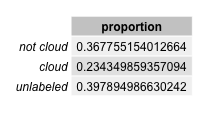
\includegraphics[width=0.325\textwidth]{1-2-1.png}
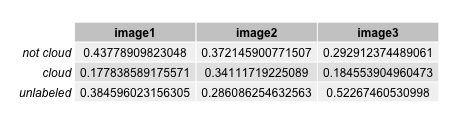
\includegraphics[width=0.665\textwidth]{1-2-2.png}
\caption{Proportion of Pixels for Different Classes}
\label{fig:1-2-1}
\centering
\end{figure}

\subsection{Summary on Data}
Table \ref{fig:1-2-1} shows that the proportions of not cloud, cloud and unlabeled pixels are 0.37, 0.23 and 0.40 respectively across the whole three images.

Separately, non-cloud pixels have the highest proportion in image 1 and image 2. The proportion of non-cloud is always higher than that of cloud. In image 1, the difference between the proportions of non-cloud and cloud pixels is largest among three images. High CORR values to some extent implies clear weather. However, the box plot \ref{fig:1-2-2} shows image 1 has low CORR values. The reason is that image 1 has smaller SD values, which means smooth surface, and smooth cloud-free terrain surface could be classified as cloudy when computing CORR values. Moreover, in image 2, the proportion of could pixels is highest compared to other images. From the box plot, we can see that image 2 has the larger NDAI values, which coincides with the evidence of presence of clouds. 



\begin{figure}[h]
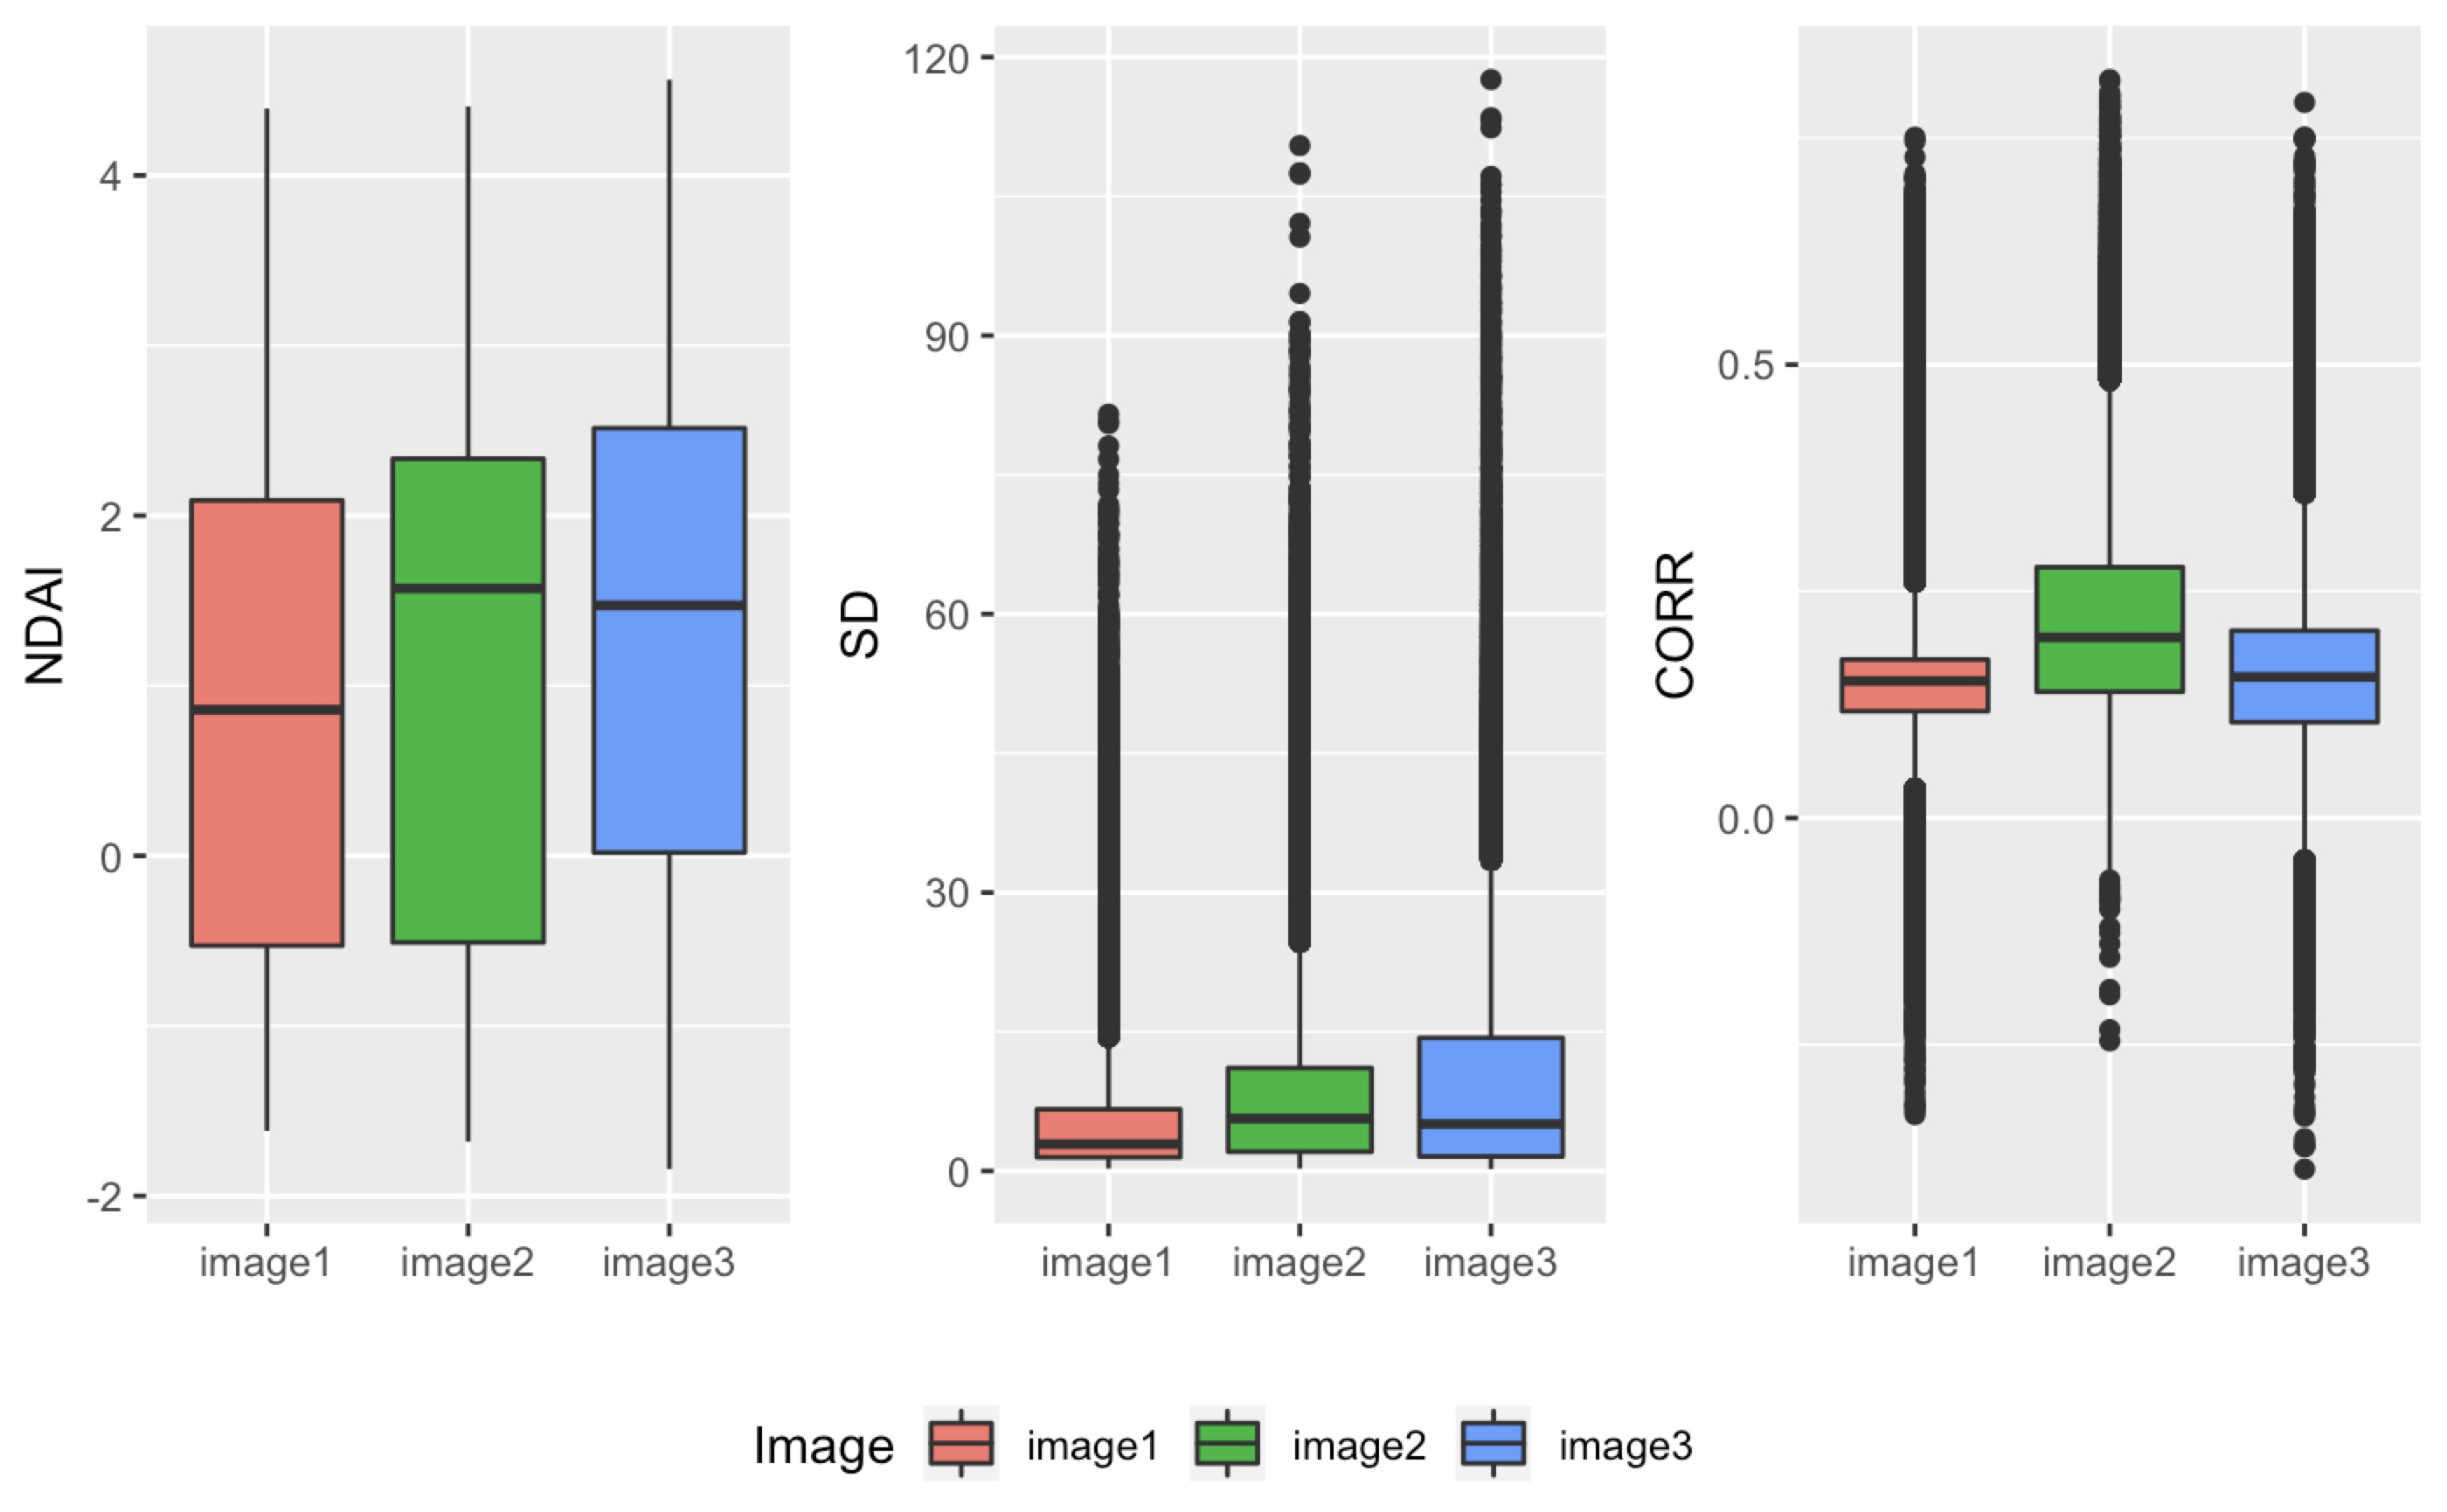
\includegraphics[width=0.49\textwidth]{1-2-3.jpeg}
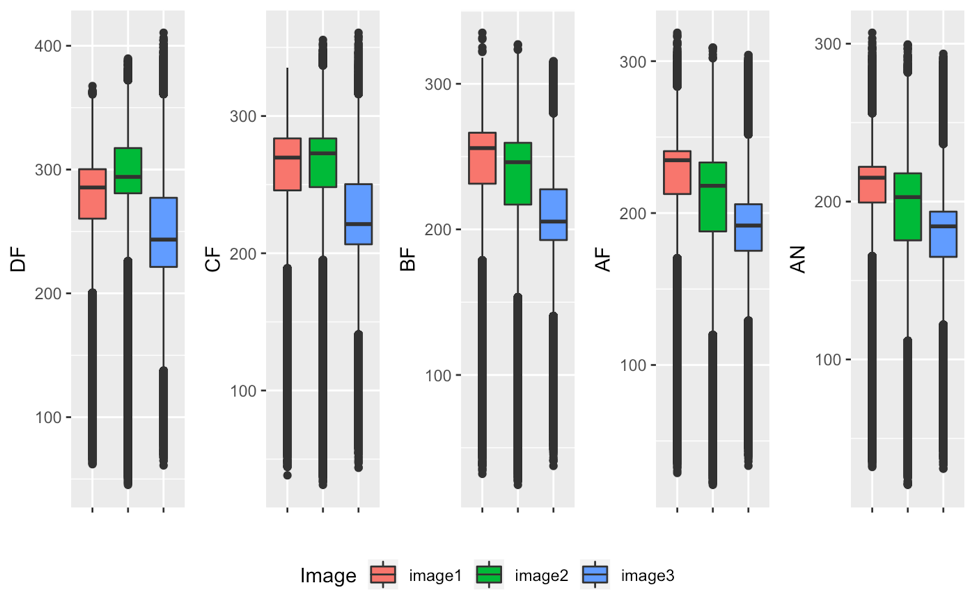
\includegraphics[width=0.50\textwidth]{1-2-3-2.png}
\centering
\caption{Box Plot}
\label{fig:1-2-2}
\centering
\end{figure}

From figure \ref{fig:1-2-3}, we can see that same label appears in proximity with each other, which indicates the samples are not identical and independent. Therefore, we cannot randomly split data into training, validation and test set. The details about data splitting is discussed in section 2.1.

\begin{figure}[h]
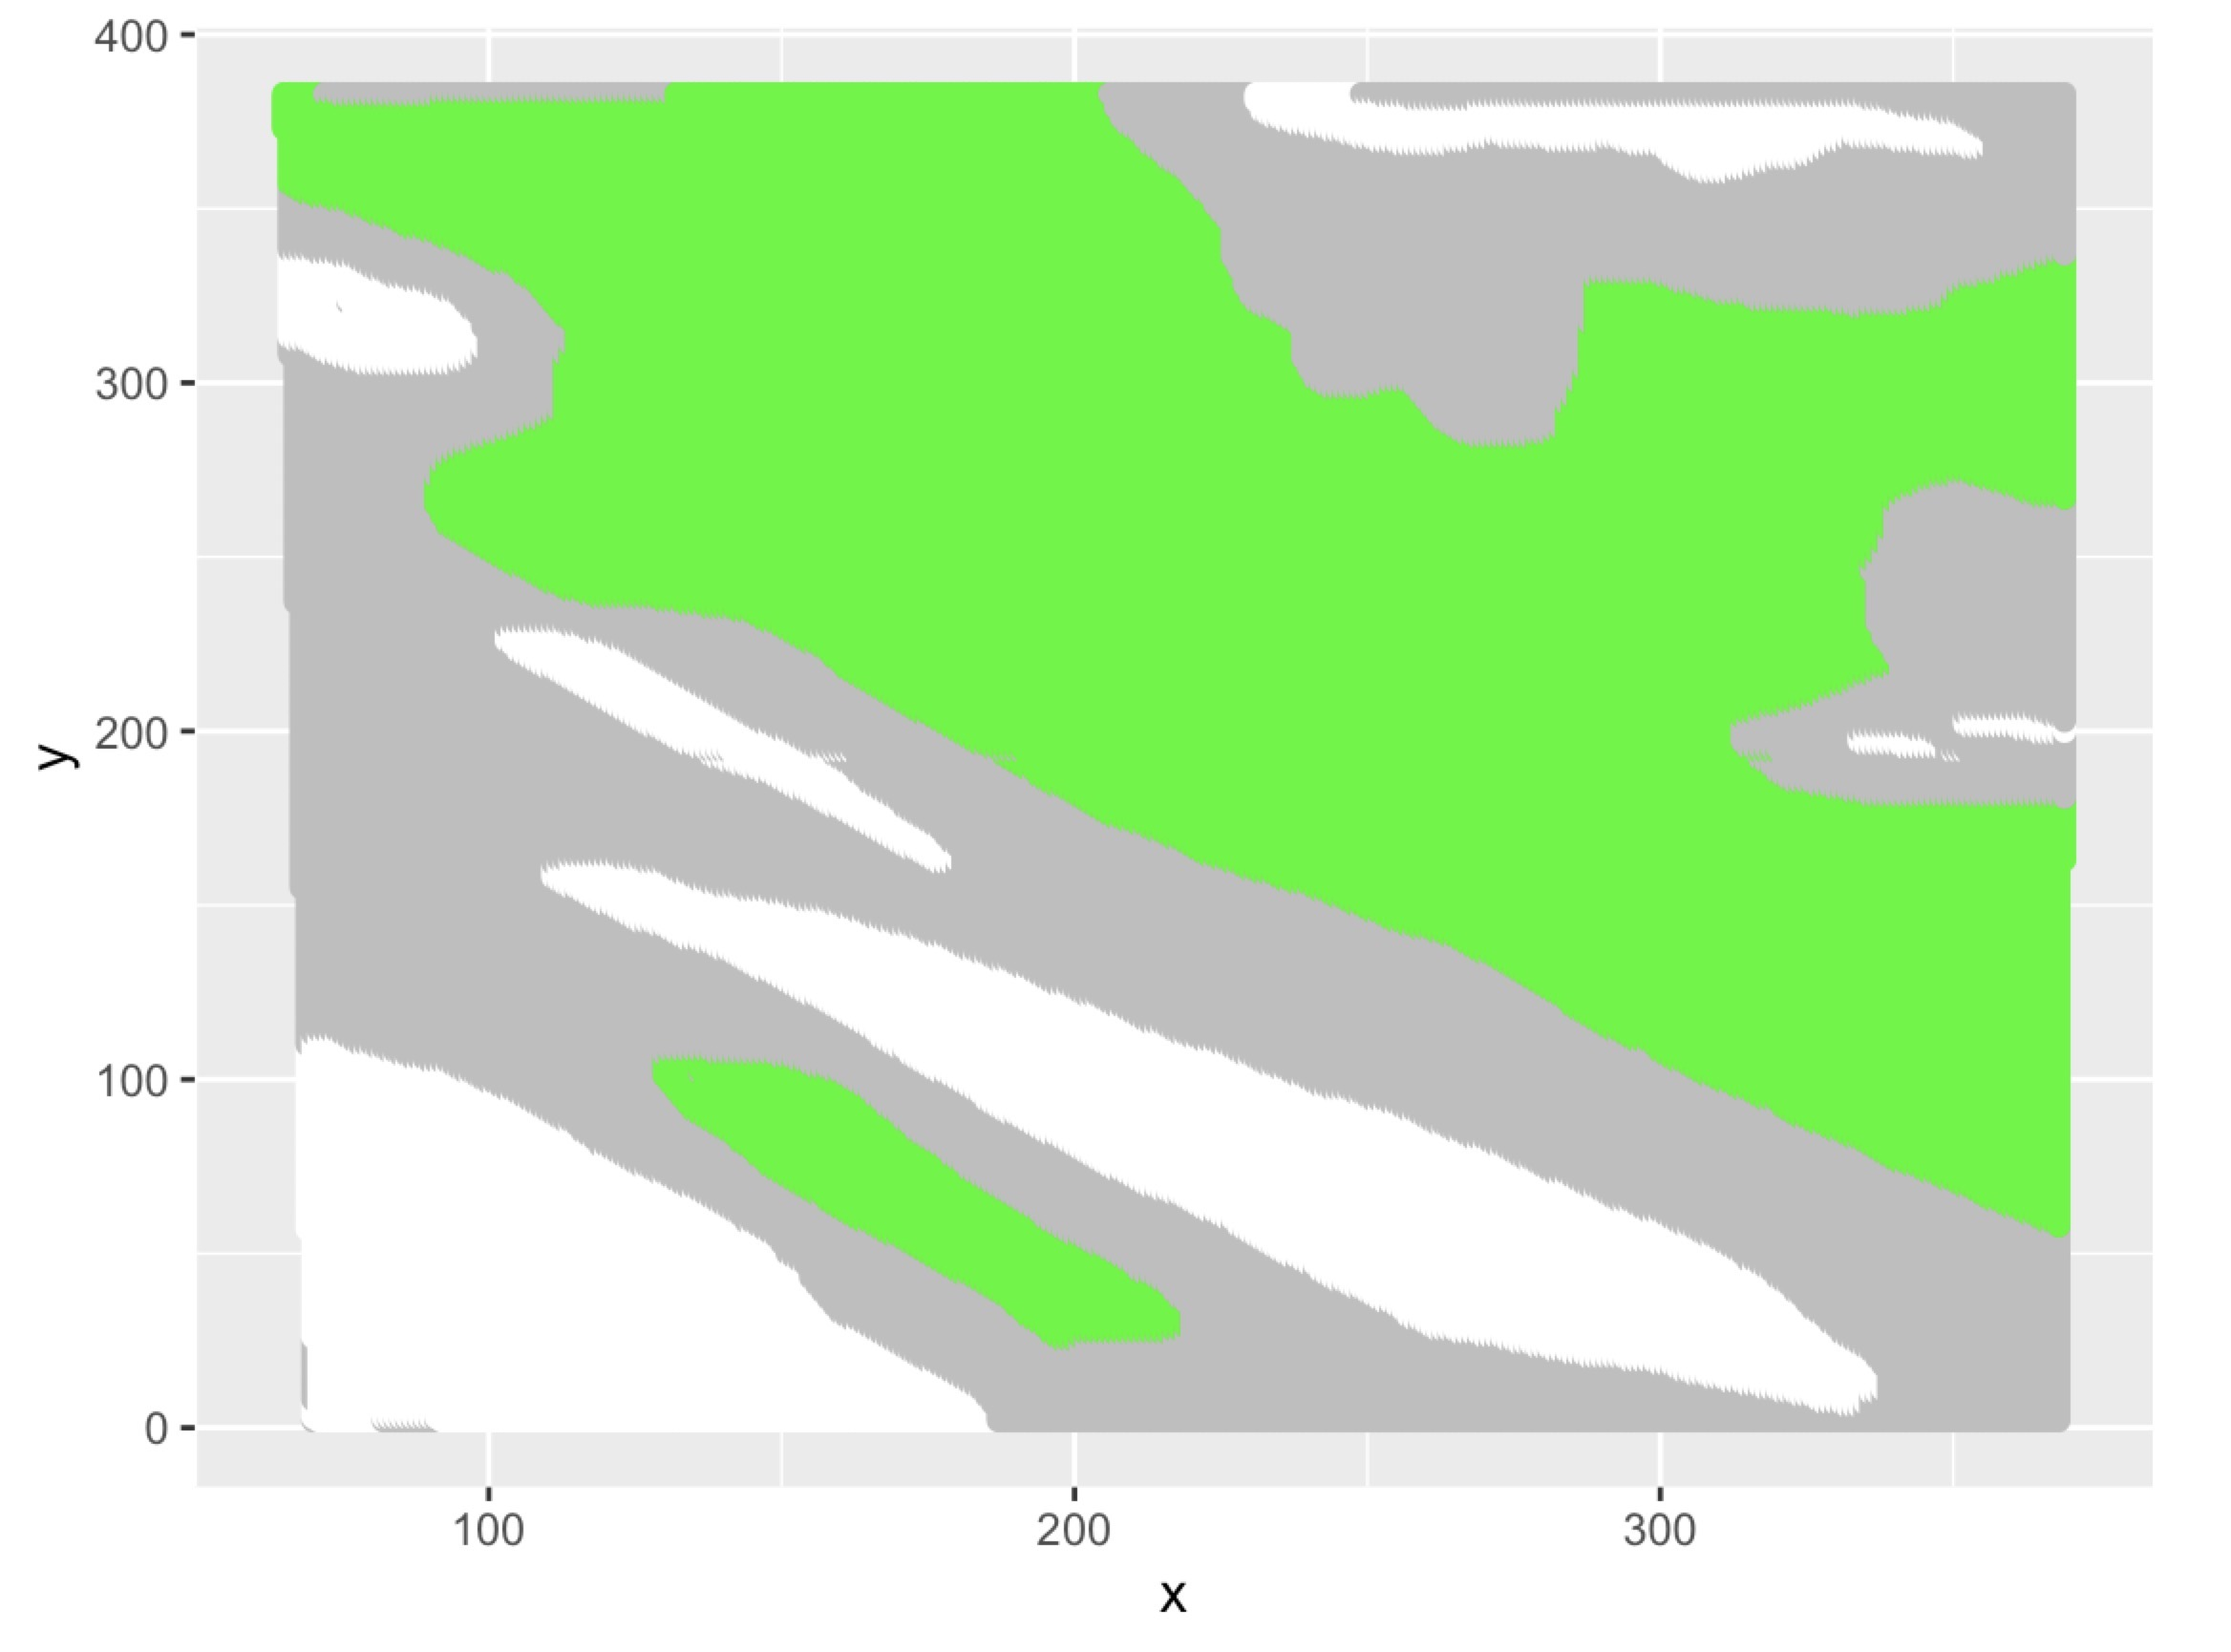
\includegraphics[width=0.31\textwidth]{1-2-4.jpeg}
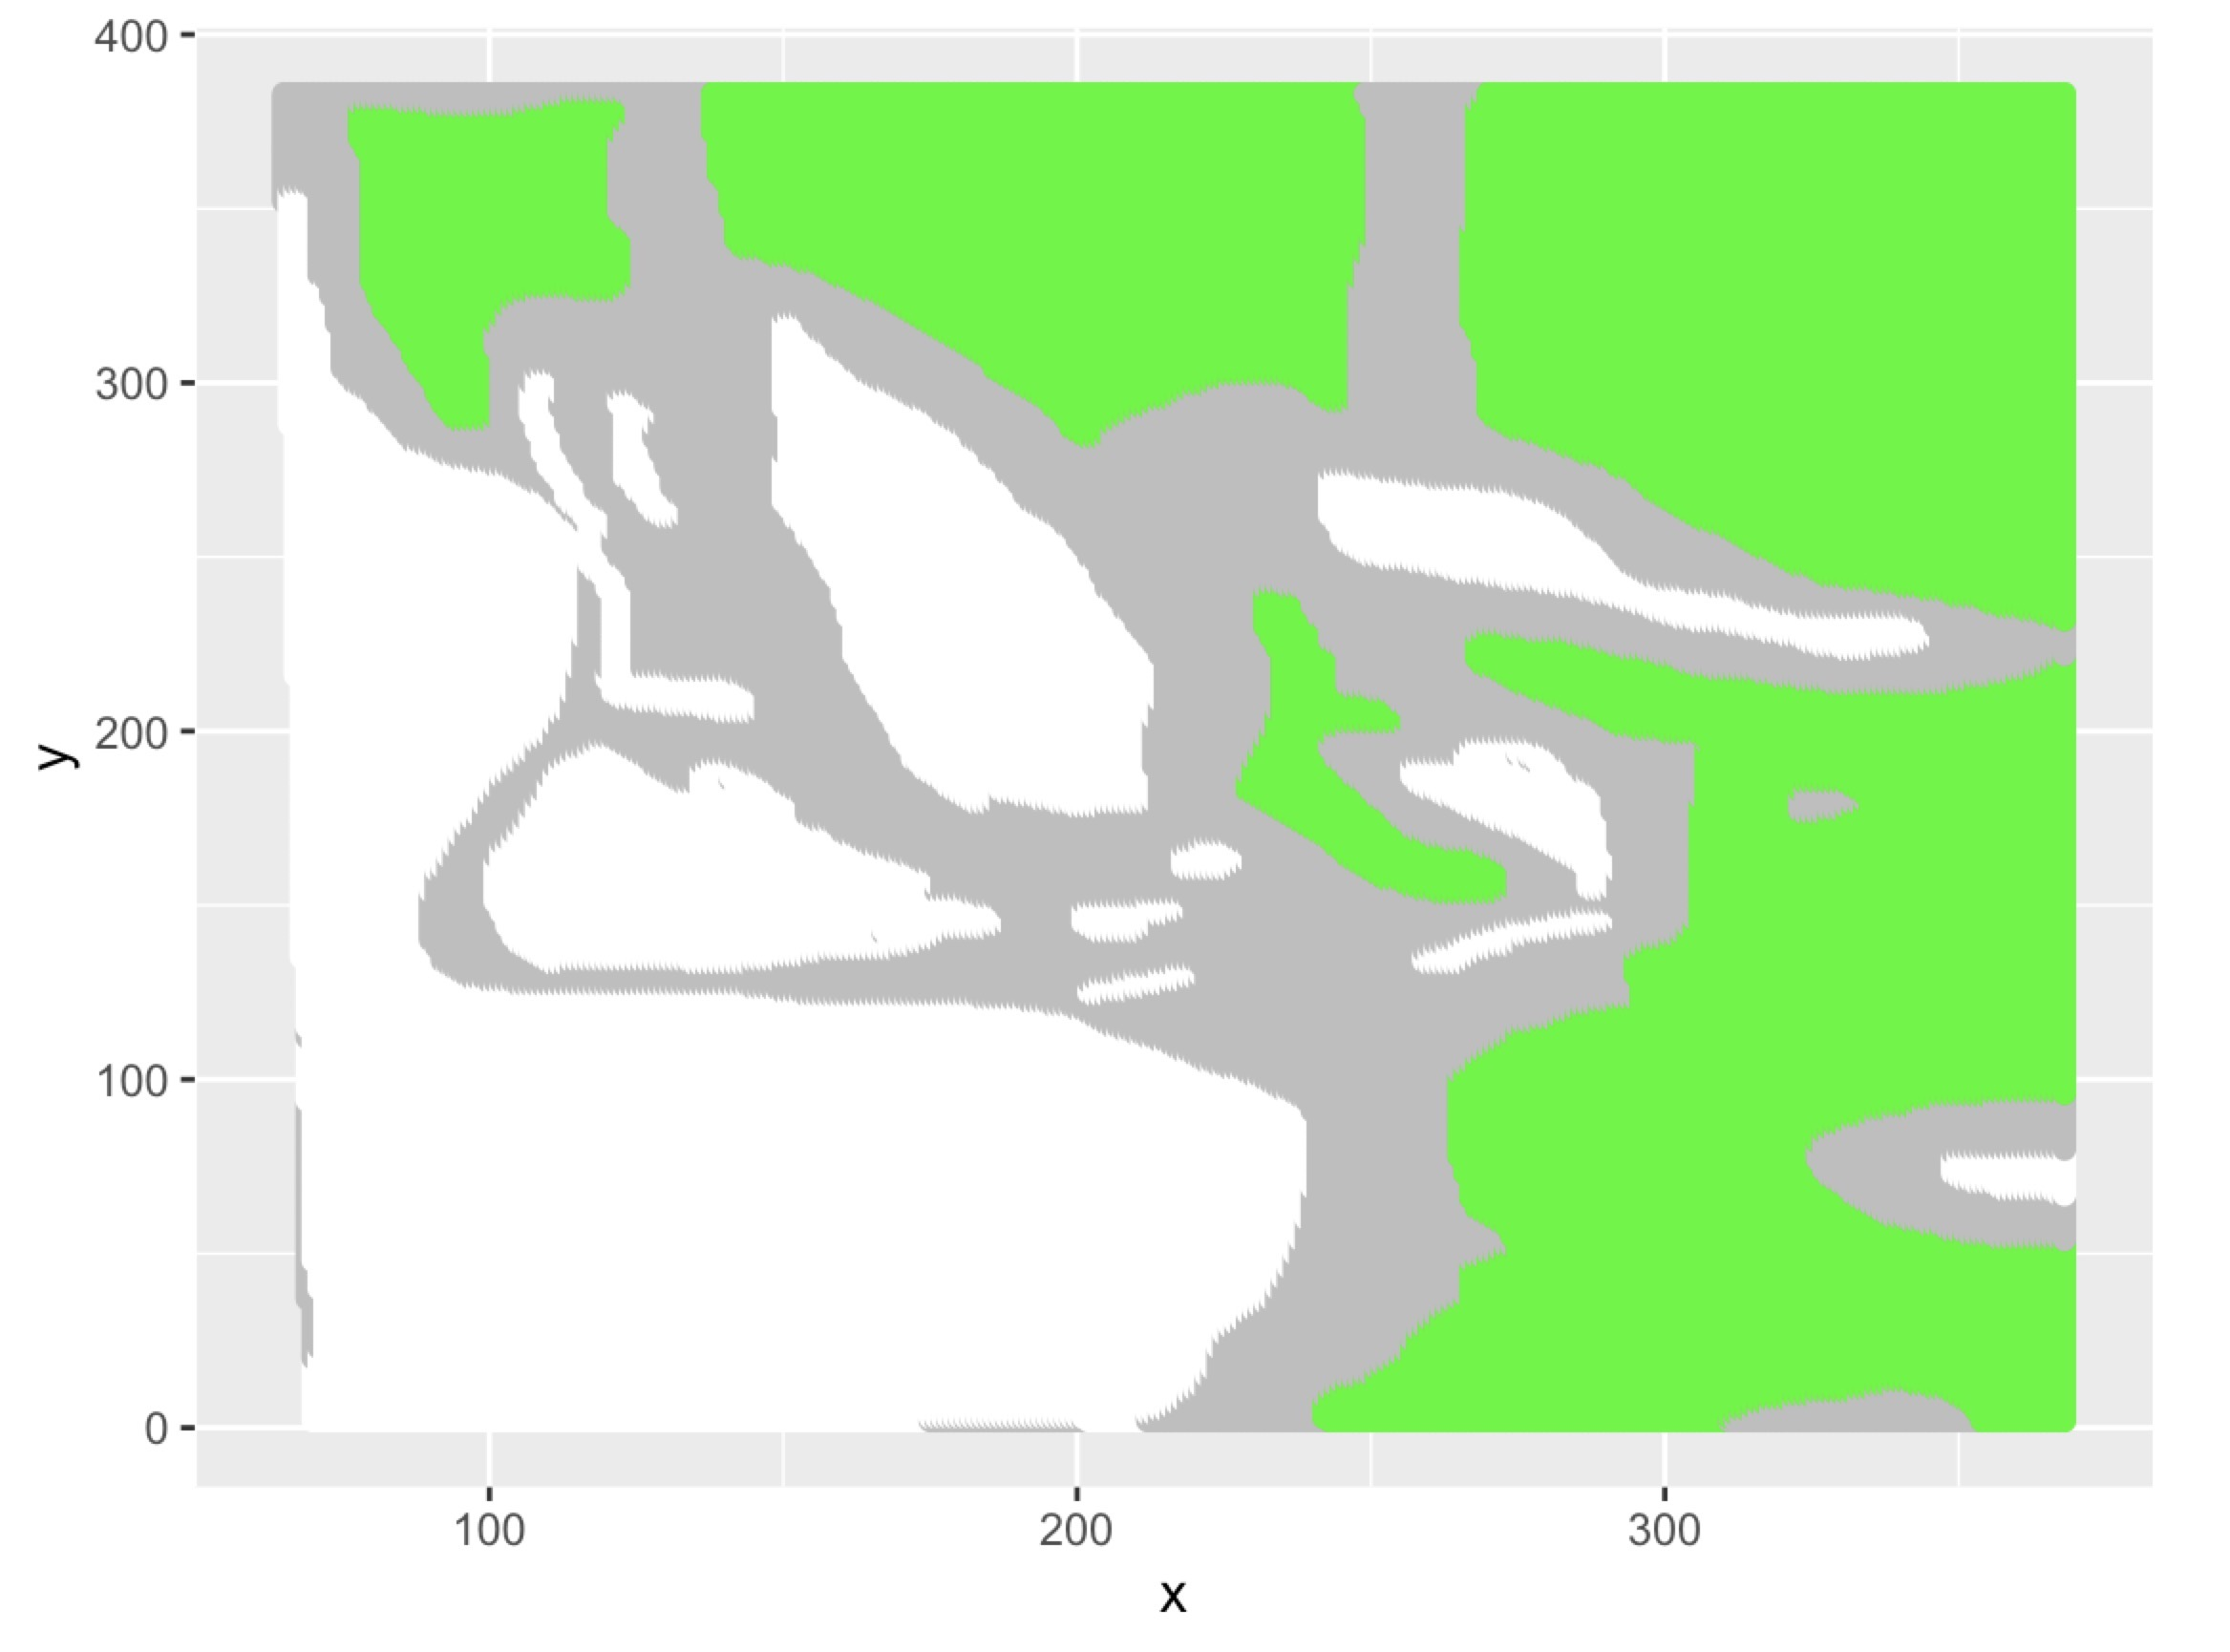
\includegraphics[width=0.31\textwidth]{1-2-5.jpeg}
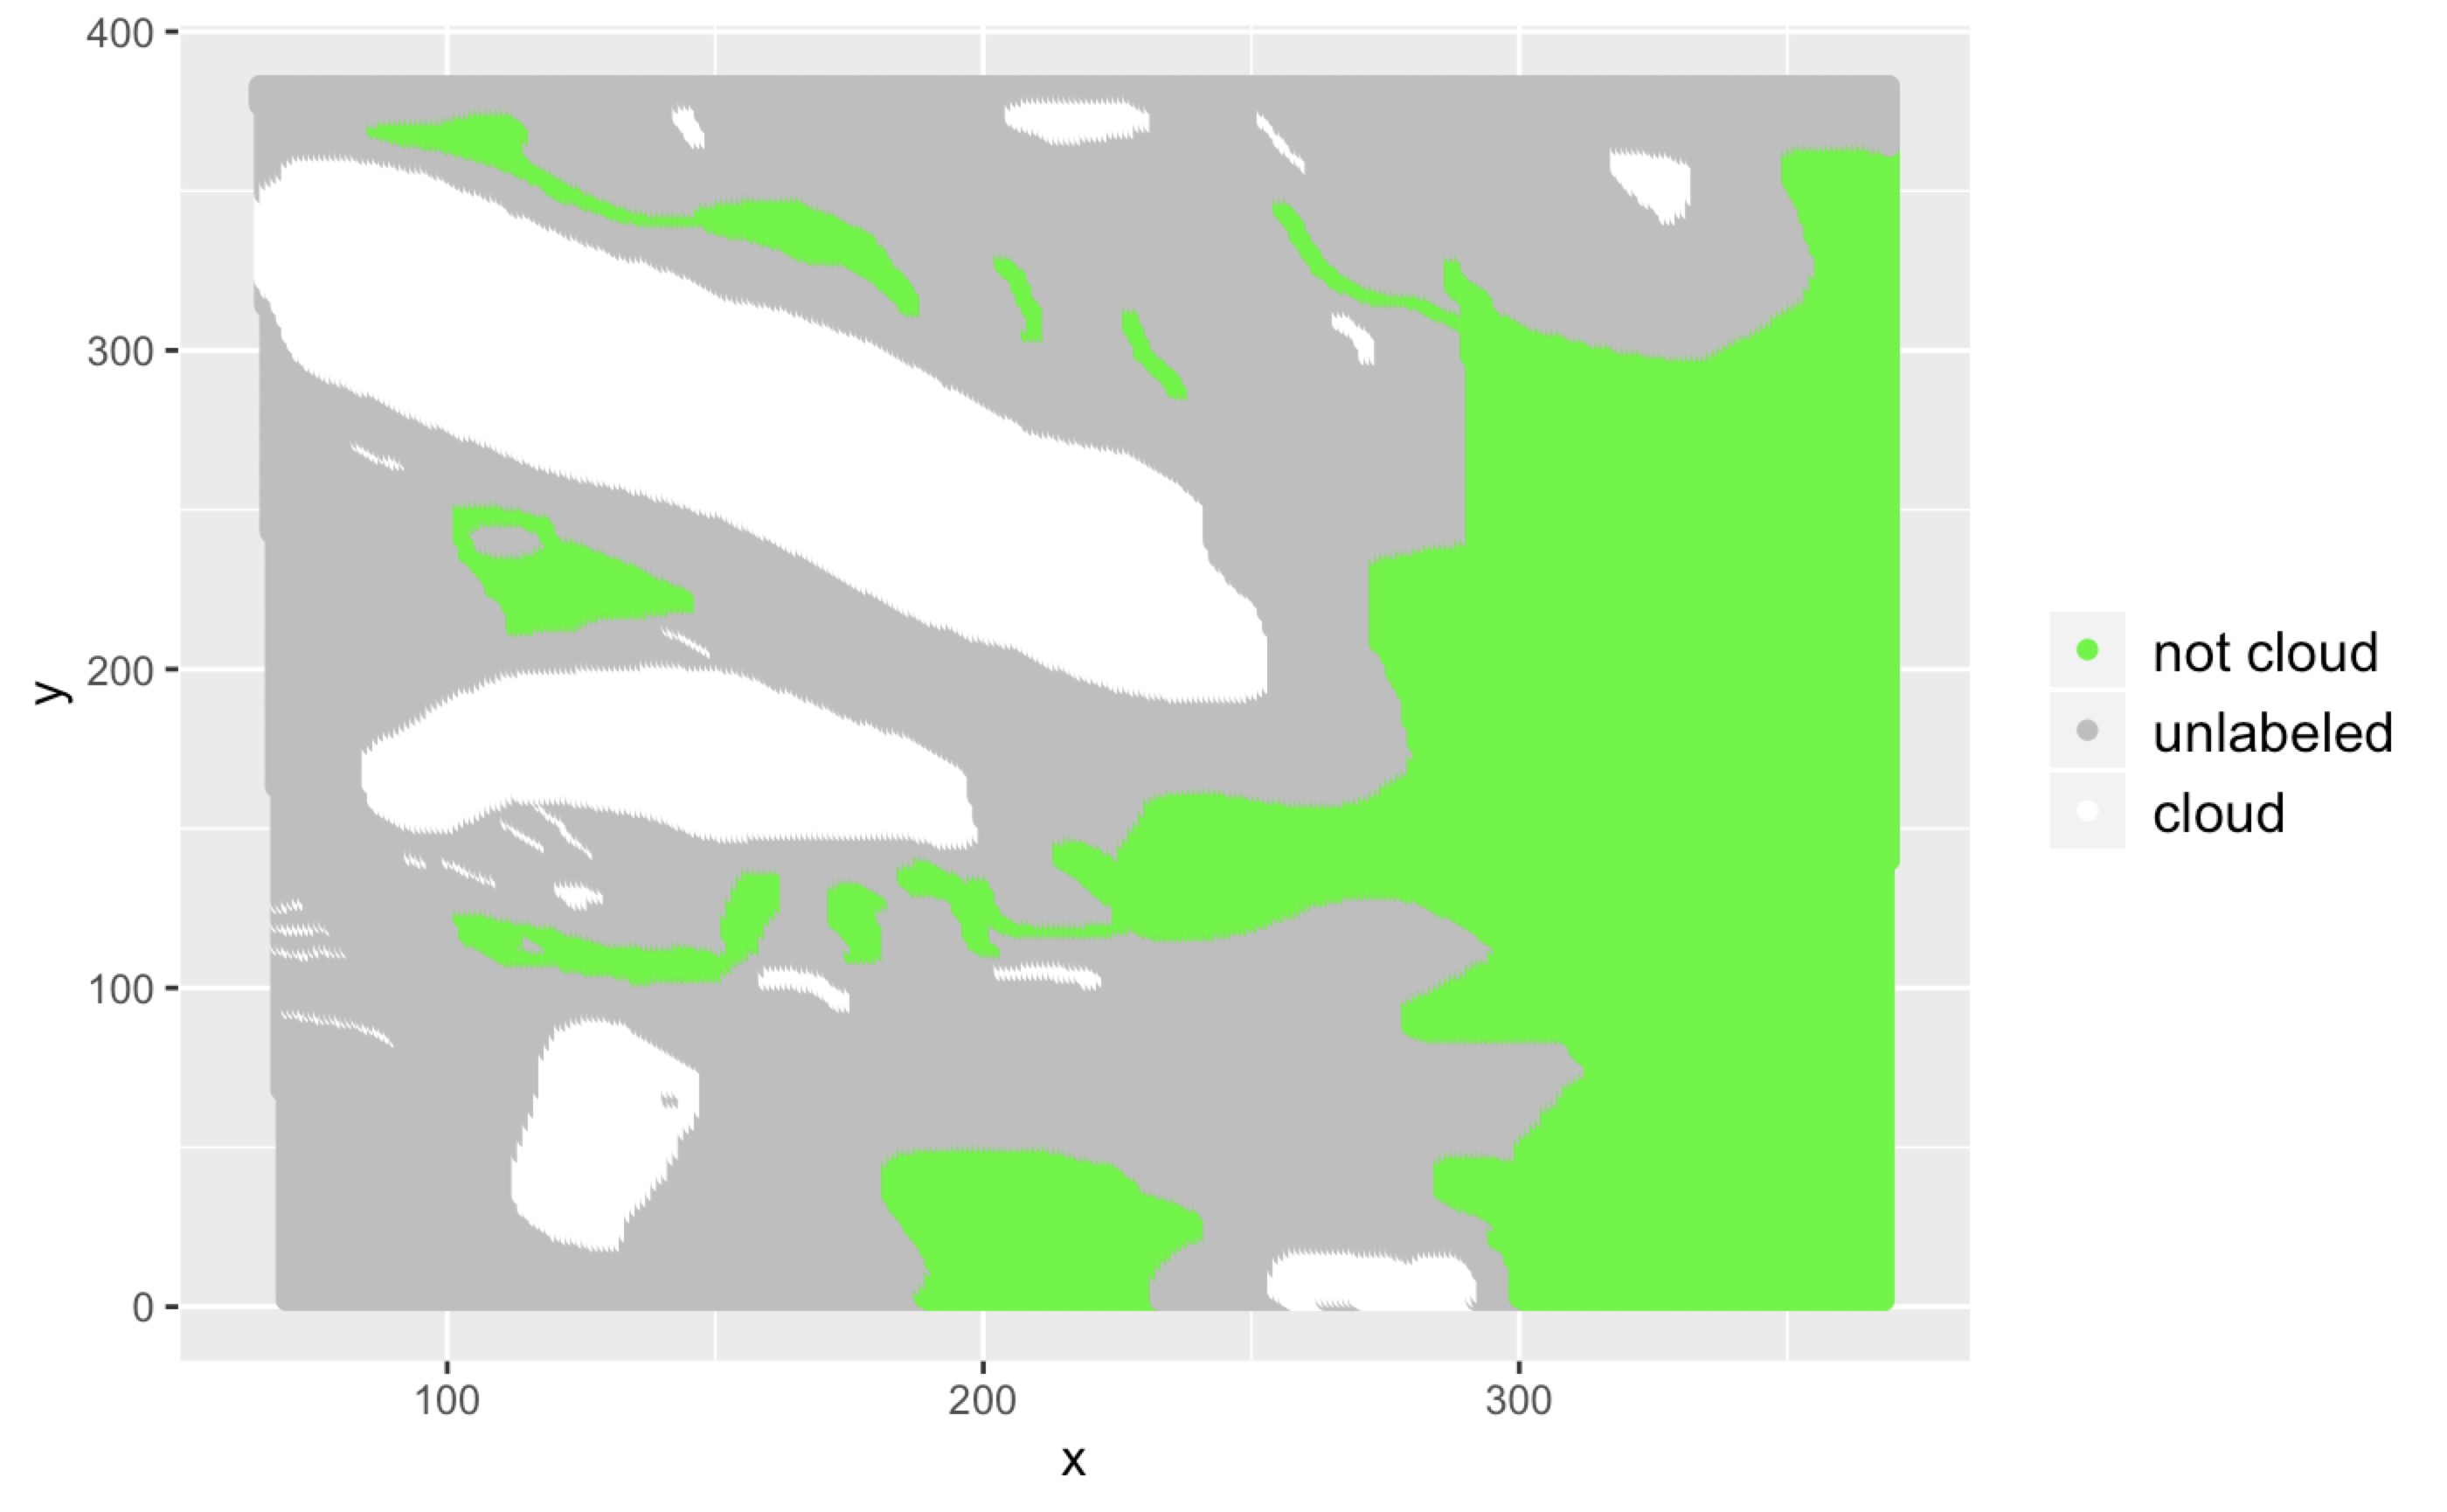
\includegraphics[width=0.37\textwidth]{1-2-6.jpeg}
\caption{Image of Expert Labels}
\label{fig:1-2-3}
\centering
\end{figure}

\subsection{EDA}

\begin{figure}[h]
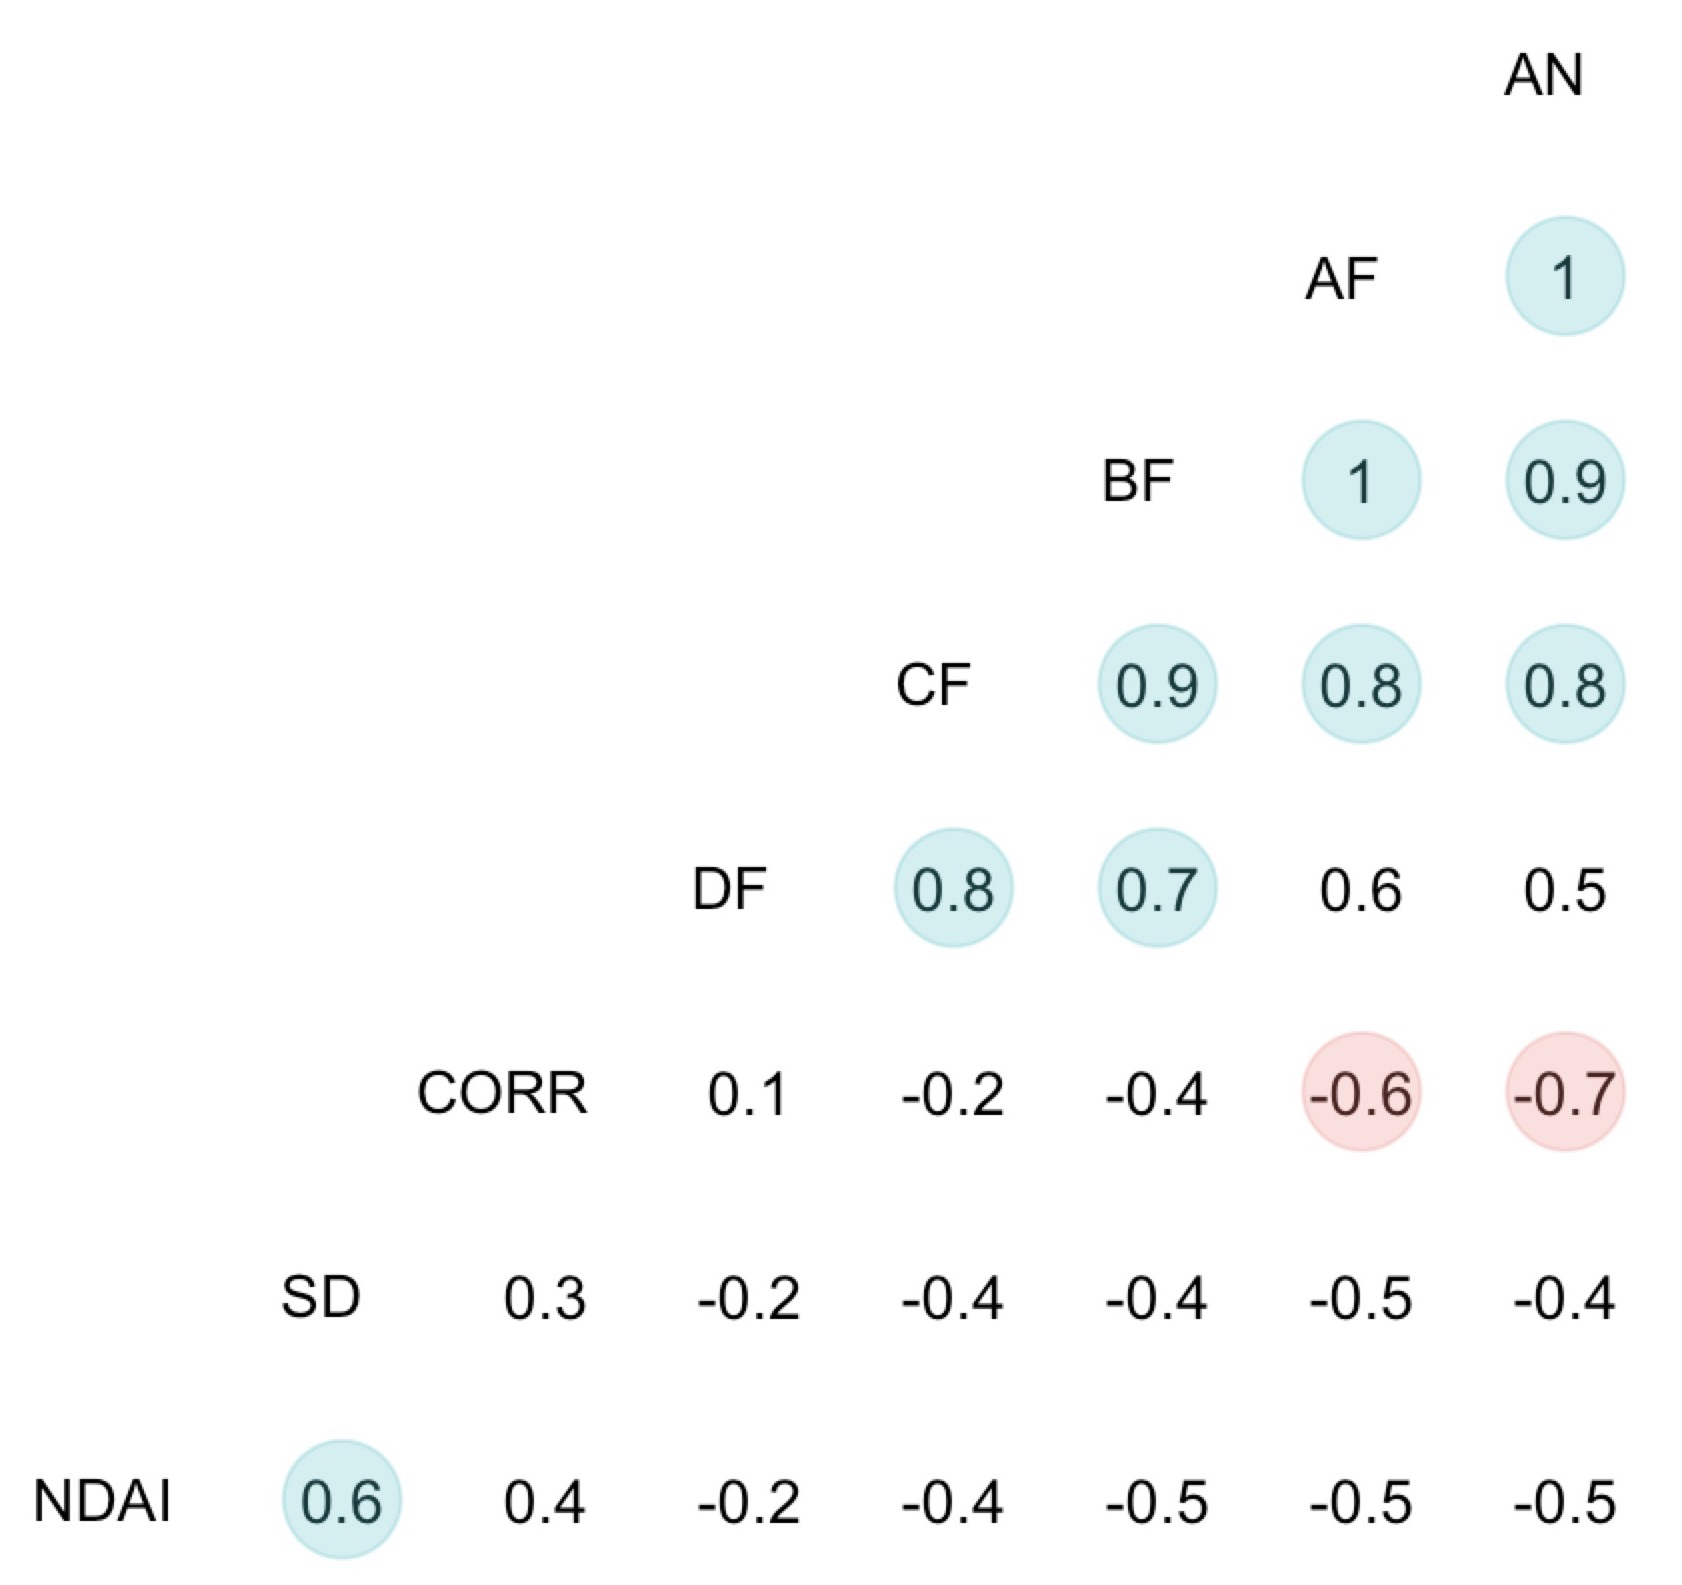
\includegraphics[width=0.4\textwidth]{1-3-1.jpeg}
\centering
\caption{Pearson Correlation Coefficient between Features}
\label{fig:1-3-1}
\end{figure}

\begin{figure}
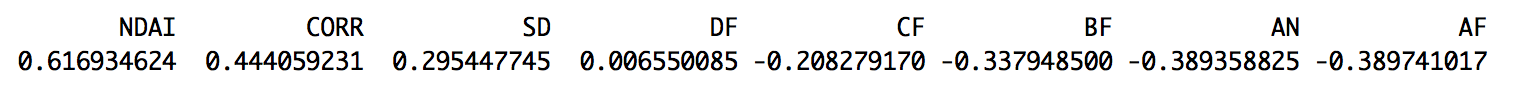
\includegraphics[width=0.9\textwidth]{1-3-2.png}
\centering
\caption{Pearson Correlation Coefficient between Response and Features}
\label{fig:1-3-2}
\end{figure}

We use Pearson correlation coefficient to measure the linear correlation. For absolute values of correlation coefficients, 0-0.19 is regarded as very weak, 0.2-0.39 as weak, 0.40-0.59 as moderate, 0.6-0.79 as strong and 0.8-1 as very strong correlation. 

In figure \ref{fig:1-3-1}, we color the pairs that have strong or very strong correlation. Specifically, AN has strong or very strong correlation with other 4 features, AF, BF, CF, and CORR.

Figure \ref{fig:1-3-2} shows the Pearson correlation coefficient values between label and features. With large absolute values, NDAI, CORR and AF might be the important features.






\section{Preparation}
\subsection{Data Splitting}

Considering the spatial properties of the data, as data points that are spatially close to each other tends to have the same labels, we need to propose some data splitting method that takes into account of the non-i.i.d (independent and identically distributed) nature of the data and try to keep the shape in whole. 

The first method would be a horizontal slice. Depending on the percentage of data split into test, validation, and training set, we apply the same percentage on the y-coordinate and slices the data. Figure \ref{fig:2-1-1} on the left shows how the data in image1 is sliced into 20\% test, 10\% validation, and 70\% train. By splitting the data with this method, we reserved the integrity of the image. The individual test, validation, and train data set after splitting are shown in Figure \ref{fig:2-1-2}.

\begin{figure}[h]
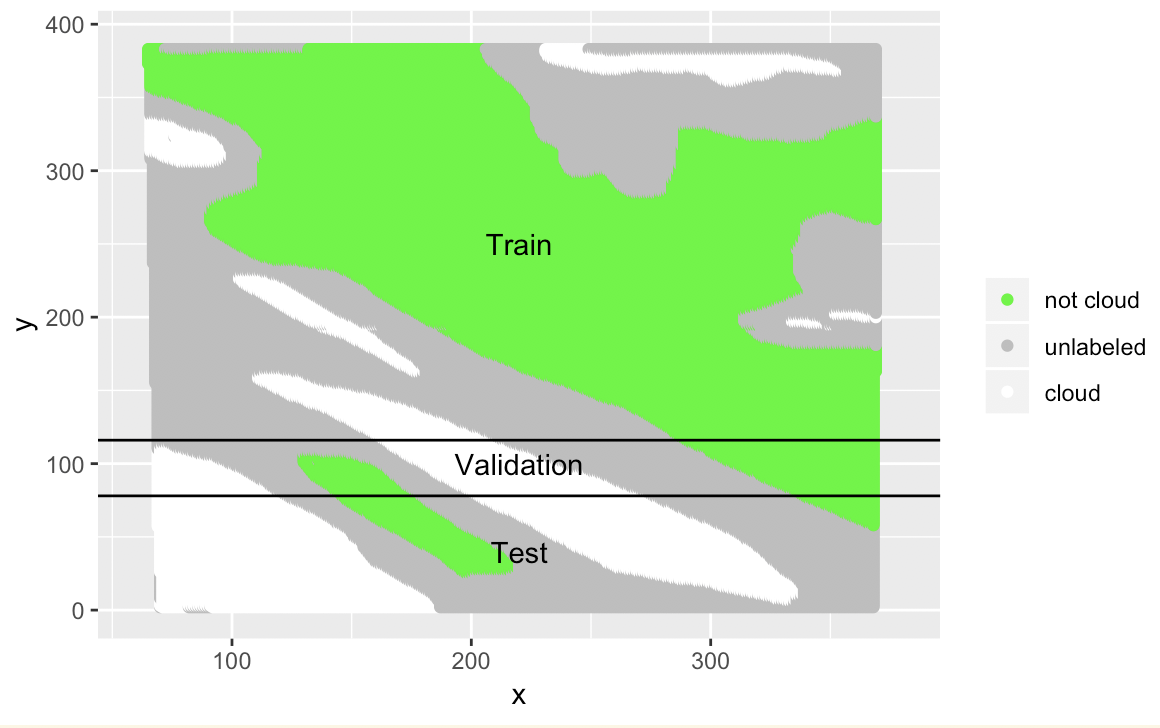
\includegraphics[width=0.4\textwidth]{2-1-1.jpeg}
\centering
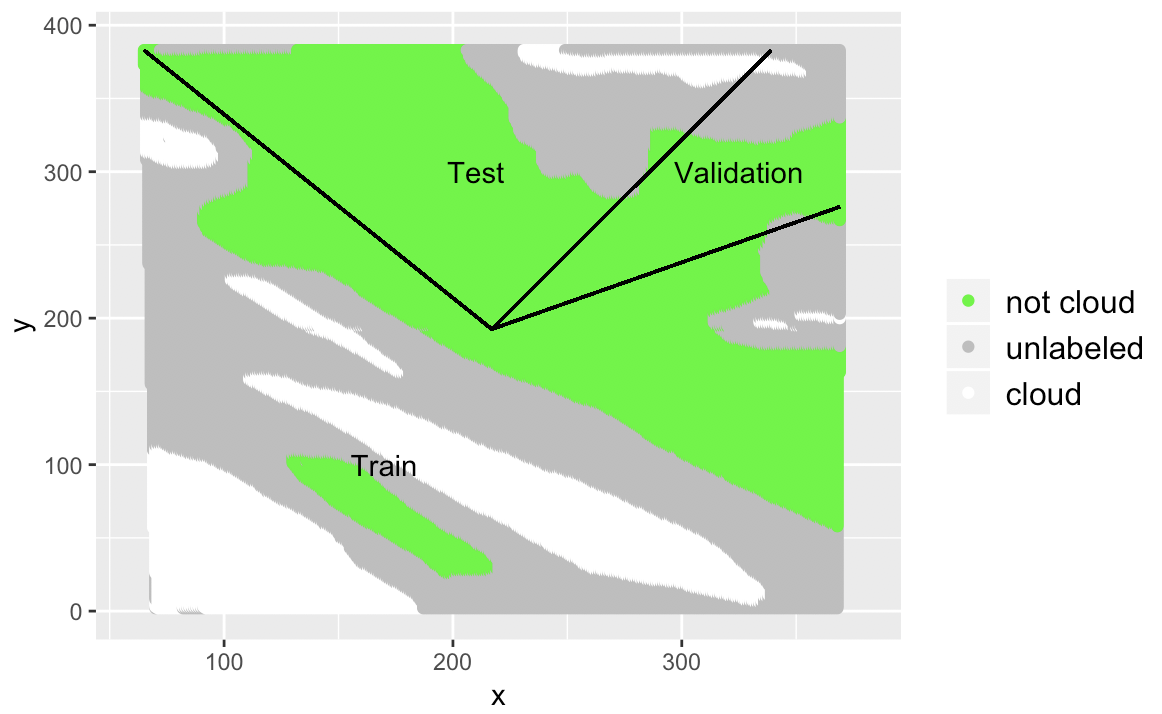
\includegraphics[width=0.4\textwidth]{2-1-2.jpeg}
\centering
\caption{Left: Method 1; Right: Method 2}
\label{fig:2-1-1}
\centering
\end{figure}

\begin{figure}[h]
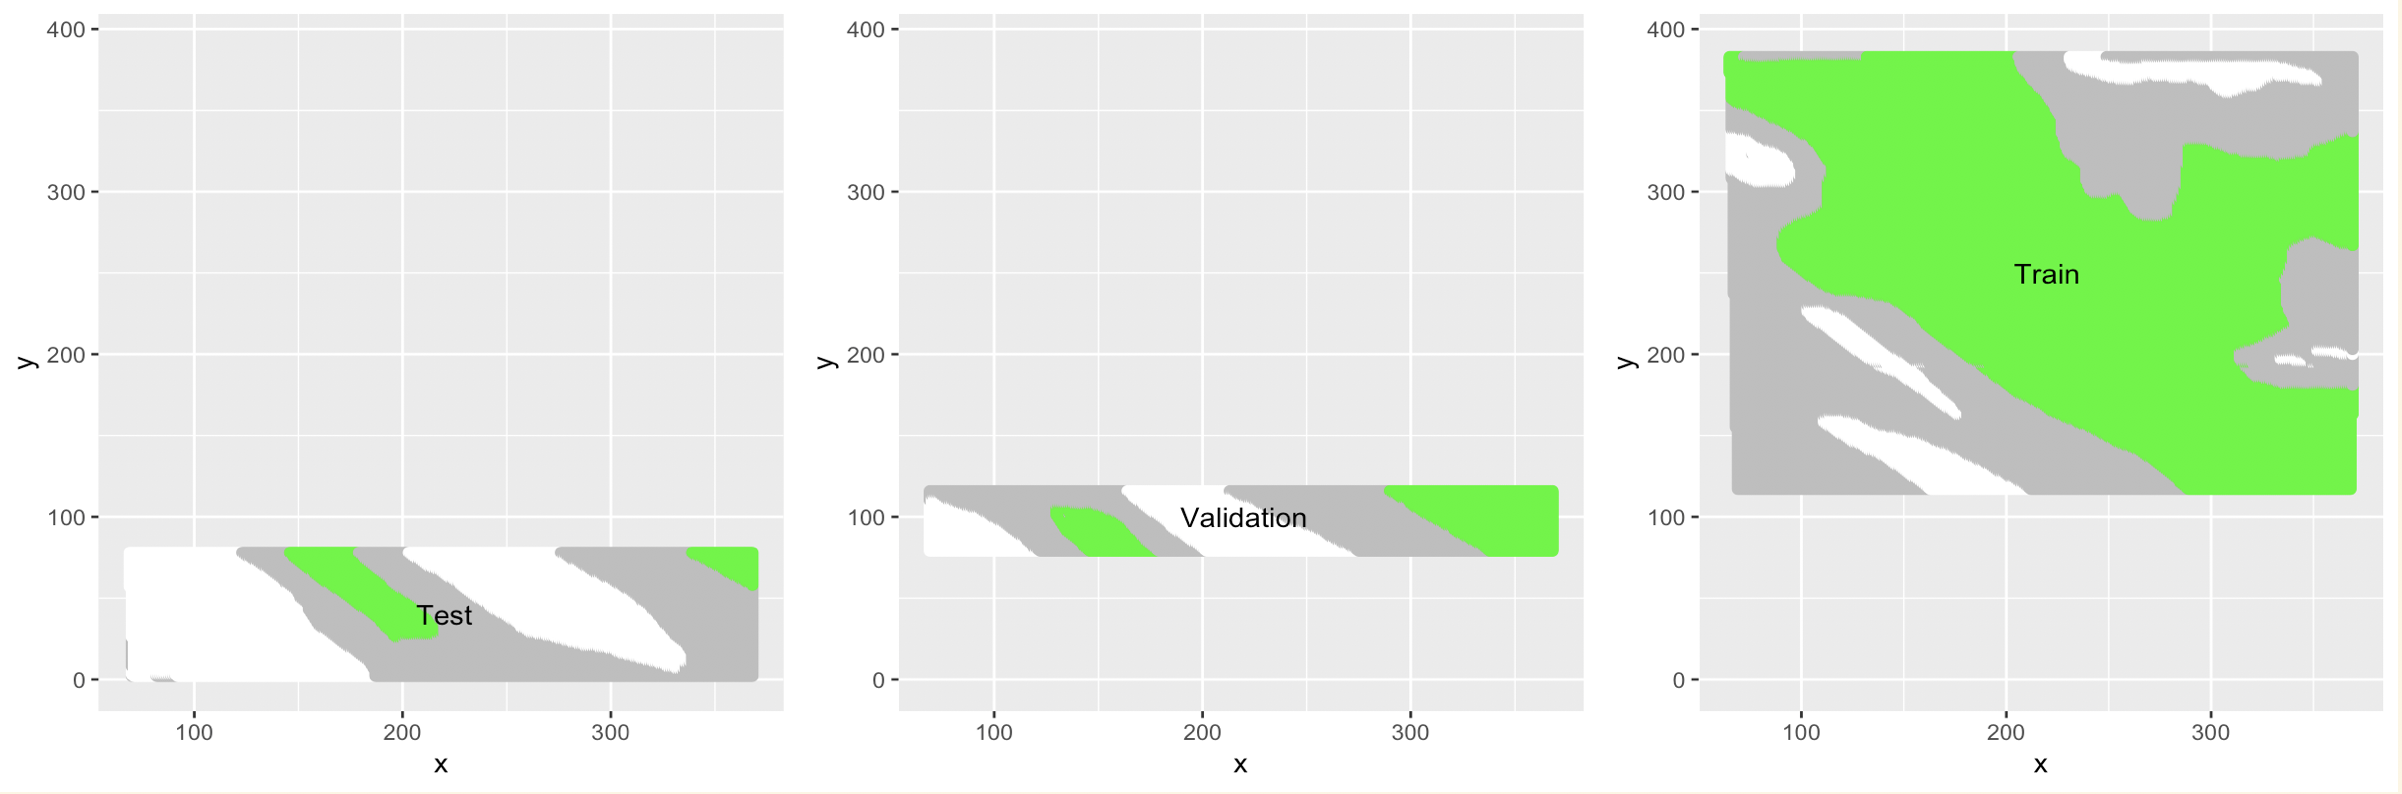
\includegraphics[width=0.8\textwidth]{2-1-3.jpeg}
\centering
\caption{Data Split with Method 1}
\label{fig:2-1-2}
\centering
\end{figure}

The second method would be slices radiated from the center of the image, much like slicing a pizza (Figure \ref{fig:2-1-1} right). Assume the slices provided 20\% test, 10\% validation, and 70\% train data. We first find the center of the image, then draw a line linking the center and the upper left corner of the data. This would be the place for the first slice. Then, we start from the upper left corner, walk along the perimeter of the image clockwise, until the distance reached 20\% the length of the perimeter. This spot will then be connected to the center for another slice. The region that is now sliced out would be the test data. Lastly, we continue to walk along the perimeter until another 10\% distance is covered. Align this spot with the center for another slice, and the new region that is sliced out would be the validation data. The piece left would be the training data. 

The important assumption to make method 2 work is that the data is roughly square shaped. By connecting points on the perimeter with the center point, we create small triangles with areas proportional to the length it took on the perimeter, since their heights are the same (since the radius remains the same in squares). With this way, we can slice out the test, validation, and train data with the exact percentage of 20\%, 10\%, and 70\%, as shown in Figure \ref{fig:2-1-3}.

\begin{figure}[h]
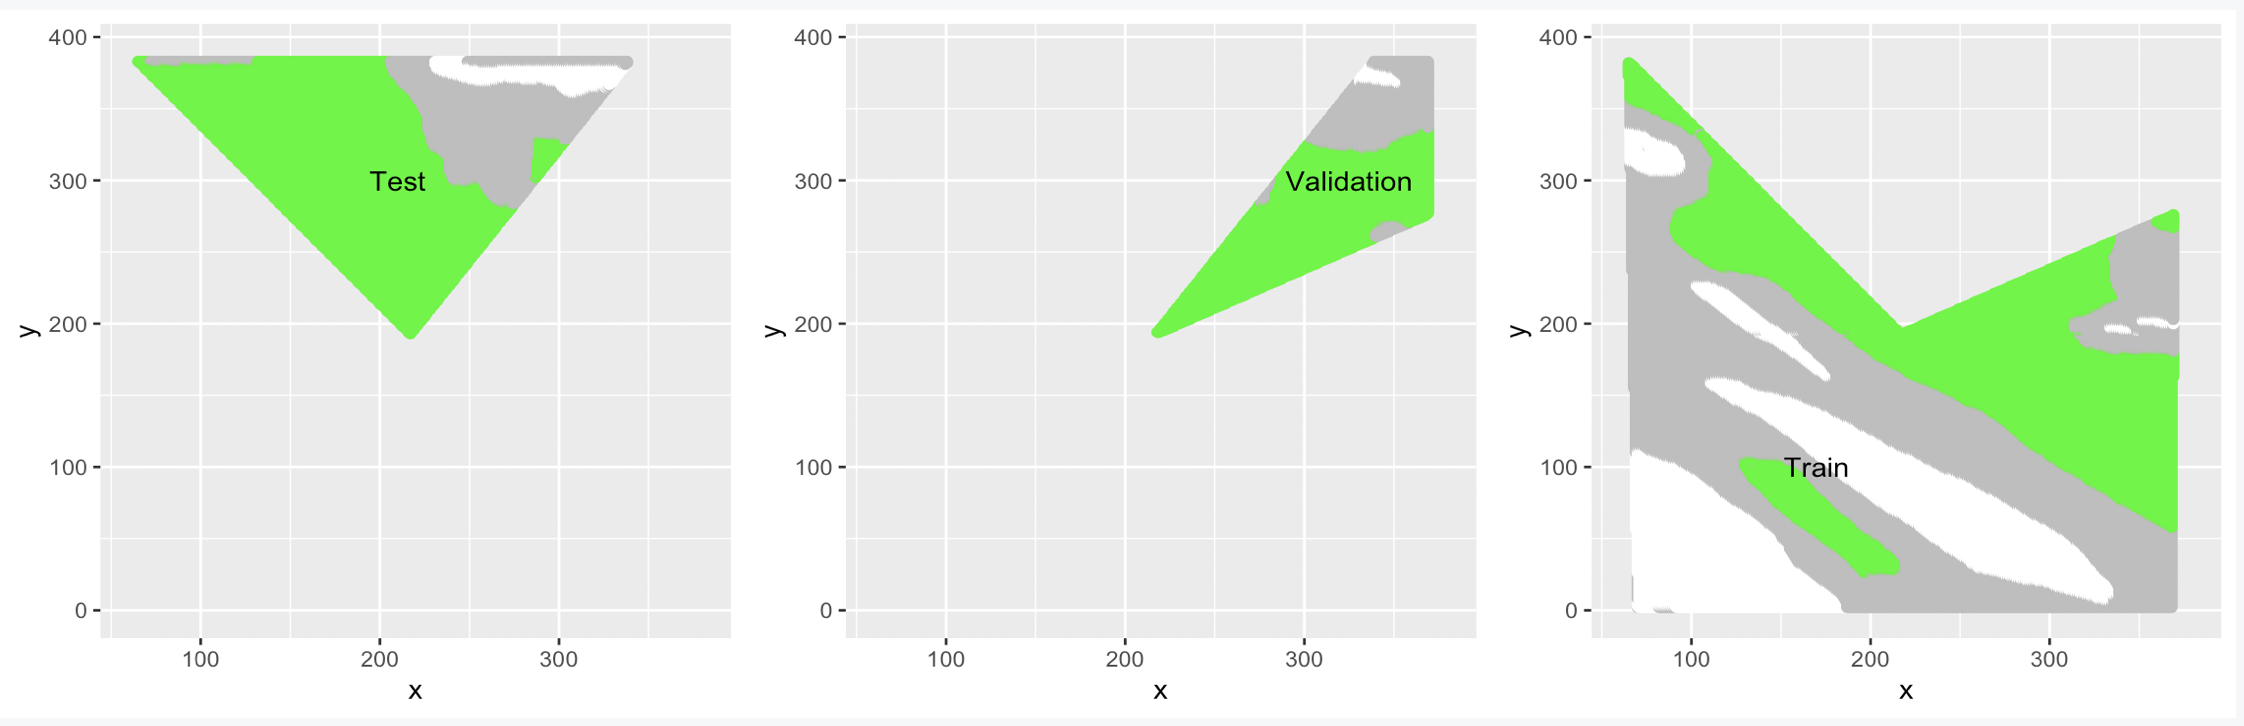
\includegraphics[width=0.8\textwidth]{2-1-4.jpeg}
\centering
\caption{Data Split with Method 2}
\label{fig:2-1-3}
\centering
\end{figure}

\subsection{Trivial Classifier}

\begin{figure}[h]
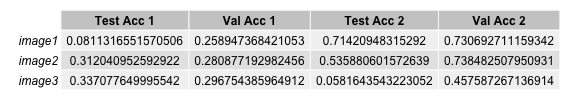
\includegraphics[width=0.8\textwidth]{2-2-1.png}
\centering
\caption{Accuracy of a Trivial Classifier}
\label{fig:2-2-1}
\centering
\end{figure}

For a trivial classifier which sets all labels to -1, its accuracy is shown in Figure \ref{fig:2-2-1}, this would be the baseline for later analysis. Since the trivial classifier sets everything to -1, it will have a high average accuracy when the expert labels are mostly -1, which means the data is skewed.

\subsection{Best Features}

We calculated the Gini Index on our data to see dividing on which variable can provide most information (the smaller gini index the better). Three of the ``best'' features are NDAI, CORR and AN with Gini Index 0.17968, 0.2841701 and 0.3499206. On the left hand side of figure \ref{fig:2-3-1}, we can see that with cut off value 0.76, NDAI has good performance to separate label 1 while CORR and AN perform well to split label -1 with cut off values 0.76 and 167.15 respectively. 


\begin{figure}[h]
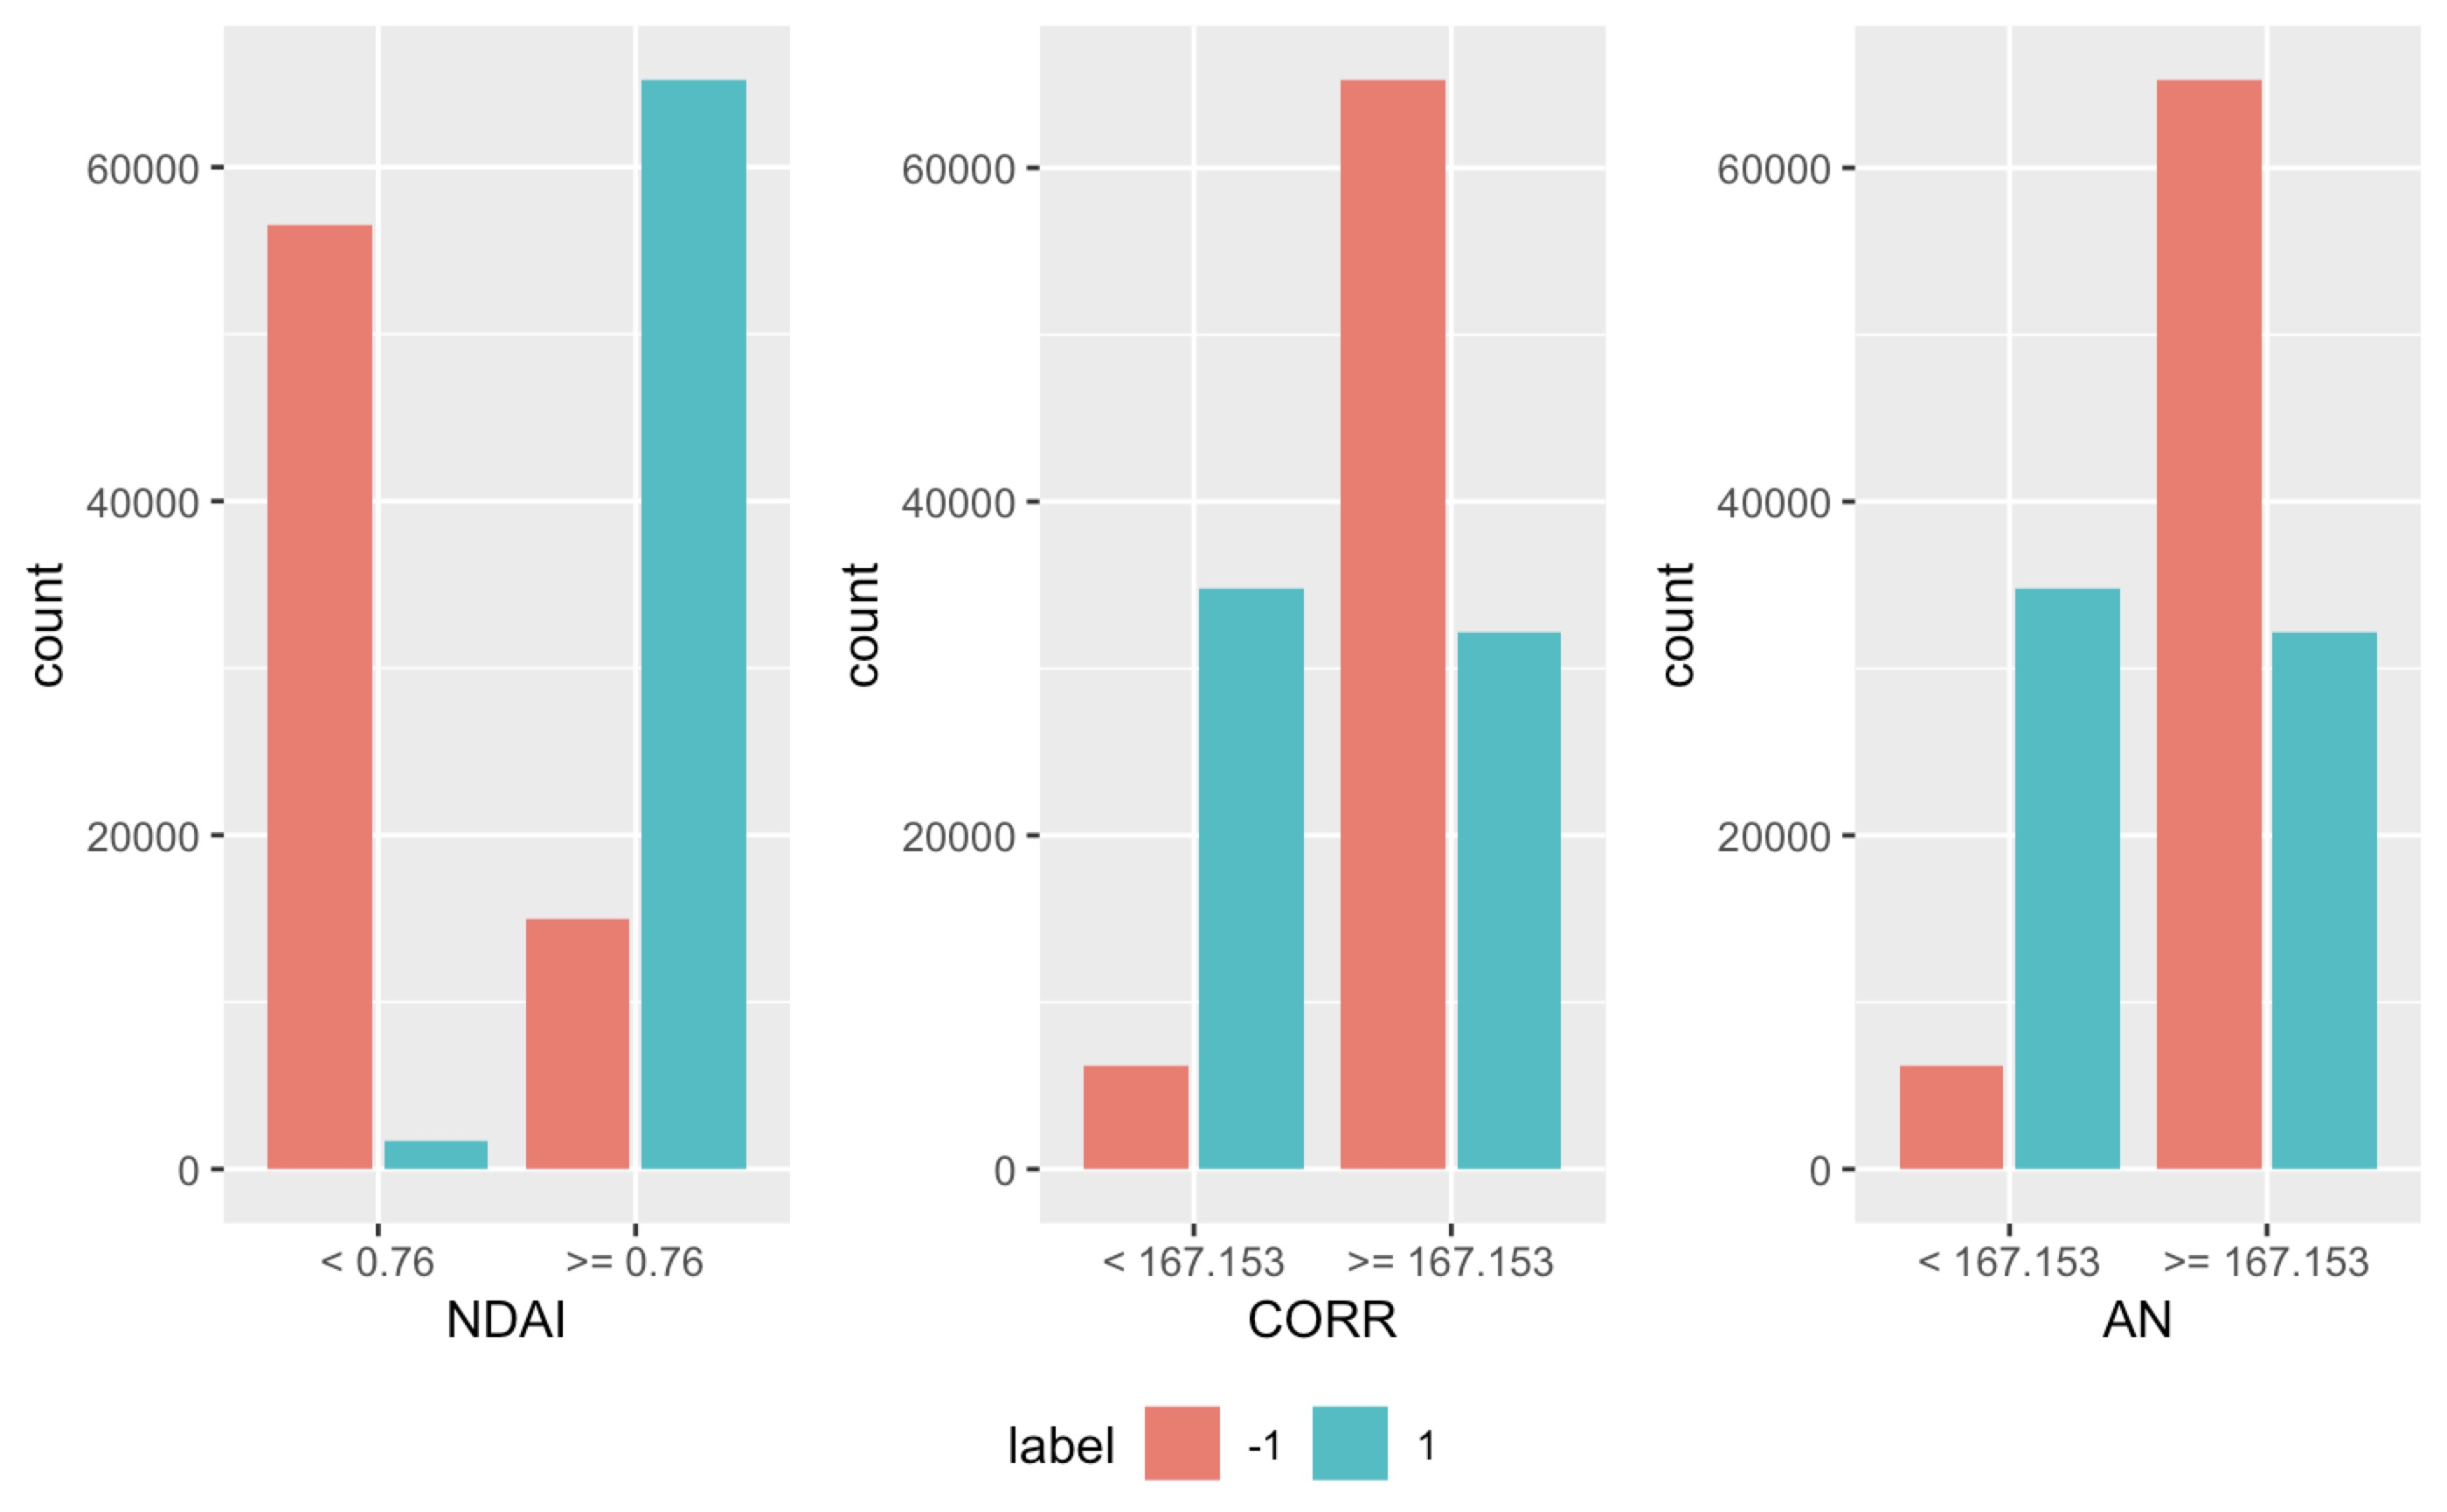
\includegraphics[width=0.5\textwidth]{2-3-1.jpeg}
\centering
\caption{Important Features}
\label{fig:2-3-1}
\centering
\end{figure}



\subsection{Cross Validation}

For each method, we implemented a general cross-validation function to do k-fold on the data with the k provided by the user, as well as the modeling function, training features, training labels, loss function, and a test data. The function trains different models according to each fold's training data, and uses its validation data to determine the best final model. The accuracy of each CV and on the test data is outputted for further review. Technically the test data set should not appear in a CV function, but for the sake of later model comparisons, we still require an input for test data and only to see how the best model across CVs performs. 

Figure \ref{fig:2-4-1} shows the plots of the training data (removed of label 0) for CV after it has been divided into 10 folds using Method 1, the horizontal slice. For each round of cross validation, one fold of data is used a validation data, and the rest are combined to provide training data. All the three images are split separately but combined together to create validation and training data.

\begin{figure}[h]
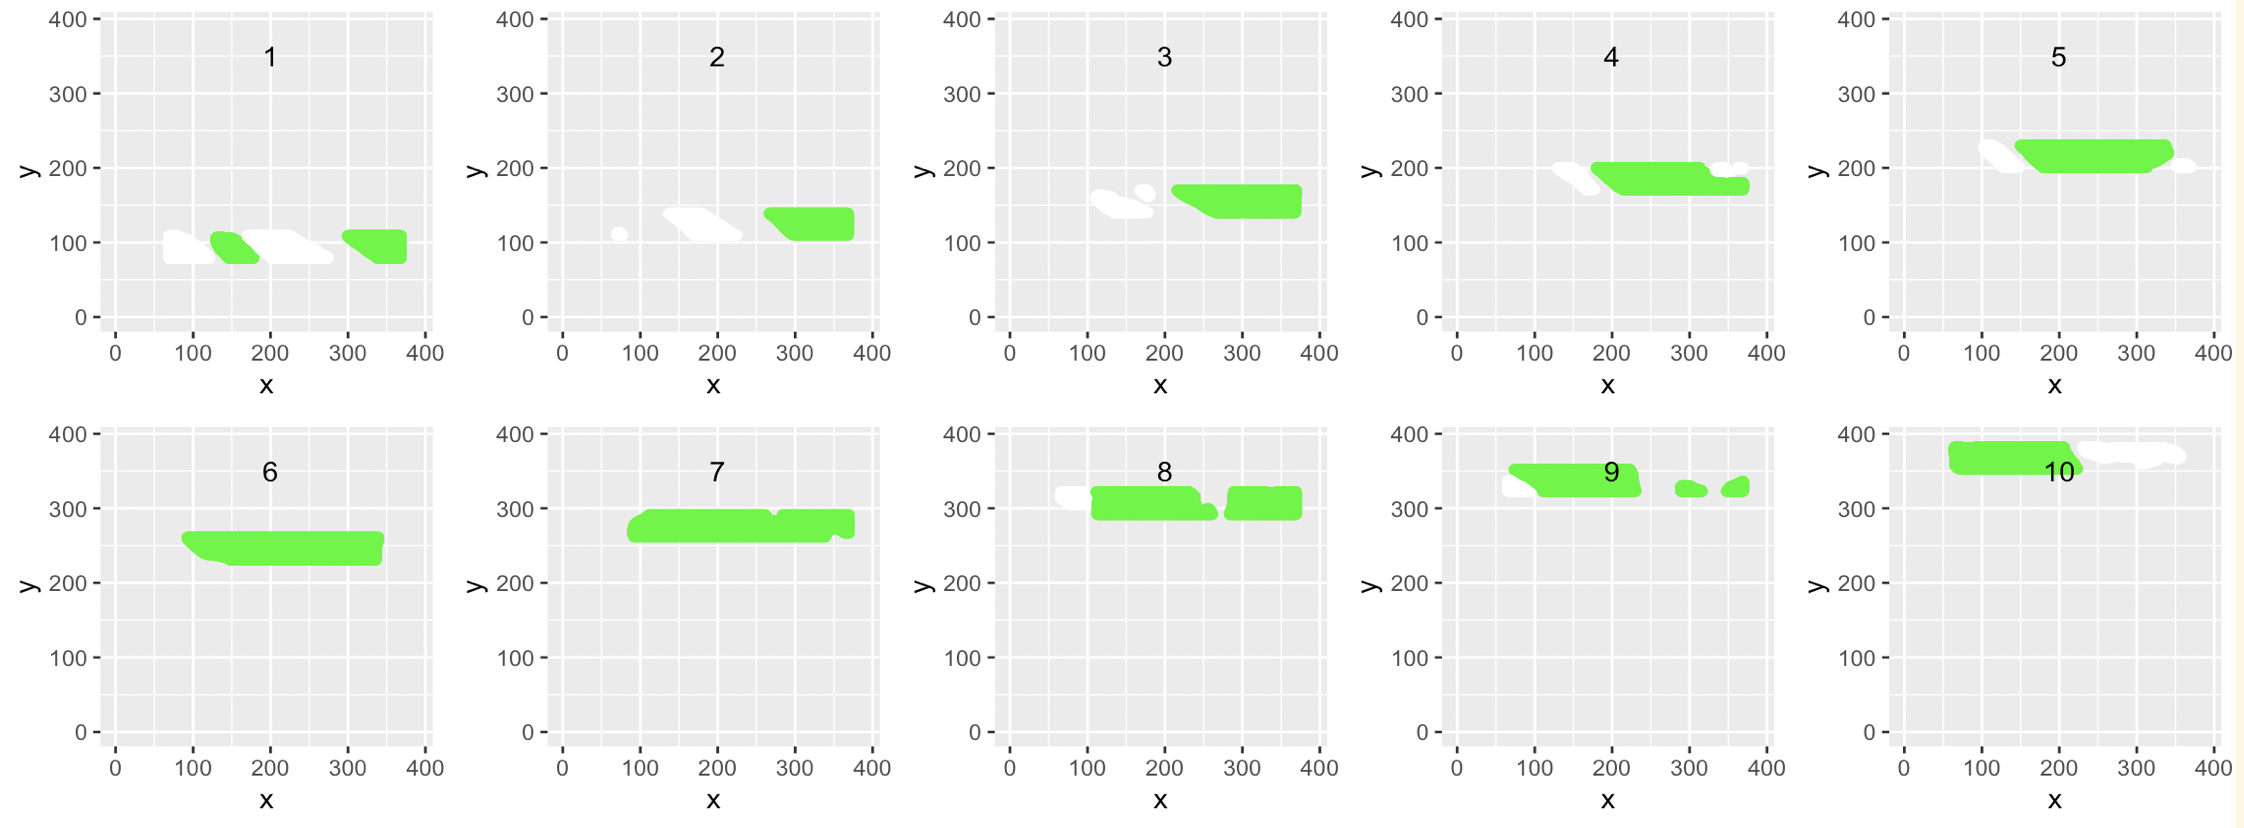
\includegraphics[width=0.8\textwidth]{2-4-2.jpeg}
\centering
\caption{Validation at Each Fold for Method 1}
\label{fig:2-4-1}
\centering
\end{figure}

Similarly, Figure \ref{fig:2-4-2} shows the plots of the training data (removed of label 0) for CV after it has been divided into 10 folds using Method 2, the ``pizza'' slice. Three images are also processed separately and combined later to make the full validation and training data. 

\begin{figure}[h]
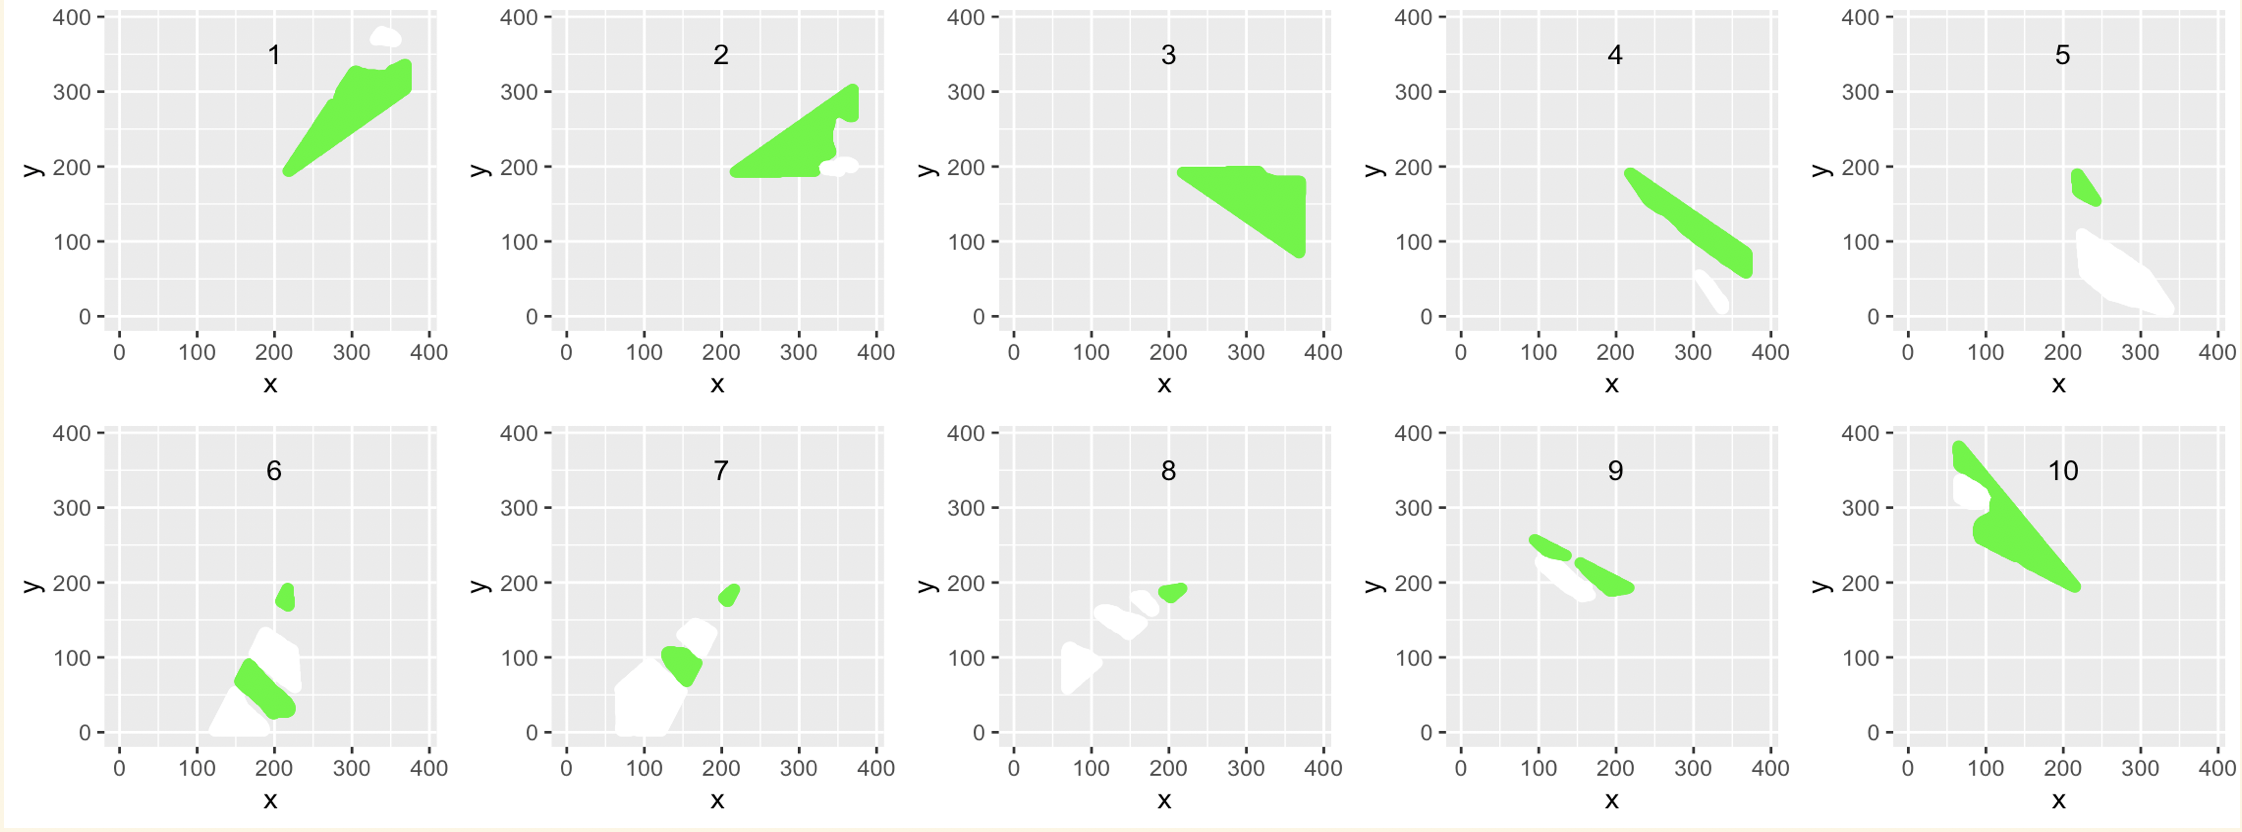
\includegraphics[width=0.8\textwidth]{2-4-1.jpeg}
\centering
\caption{Validation at Each Fold for Method 2}
\label{fig:2-4-2}
\centering
\end{figure}

The code for CV can be seen at:

https://github.com/estherwu211/stat154\_project2/blob/master/CVgeneric.Rmd

\section{Modeling}

\subsection{Logistic Regression}

A logistic regression is trained as a simple and basic model for classification, mainly serving purpose as a baseline model, in addition to the baseline we calculated in 2.2. Since logistic regression separate values with a linear line, it might not work as well as other methods that we will talk about later. All accuracy across folds for two dividing methods are shown in Figure \ref{fig:3-1-1}. Overall, logistic regression performs better than baseline. We also used ROC curves to find the optimal cutoff value for this model, and the accuracy after the updated cutoff value is shown in the lower two rows of Figure \ref{fig:3-1-1}. The ROC curve and the chosen cutoff value by Youden index is shown in Figure \ref{fig:3-1-2}. The new cutoff value is 0.02 for method 1 and 0.97 for method 2 in terms of probability.

\begin{figure}[h]
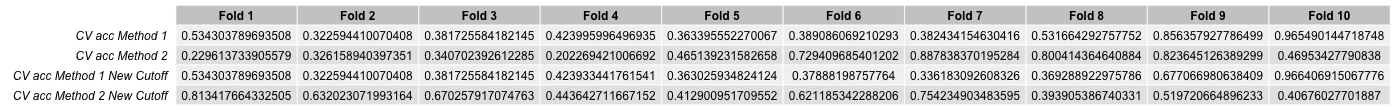
\includegraphics[width=\textwidth]{3-1-1.png}
\centering
\caption{Accuracy of Logistic Regression}
\label{fig:3-1-1}
\centering
\end{figure}

\begin{figure}[h]
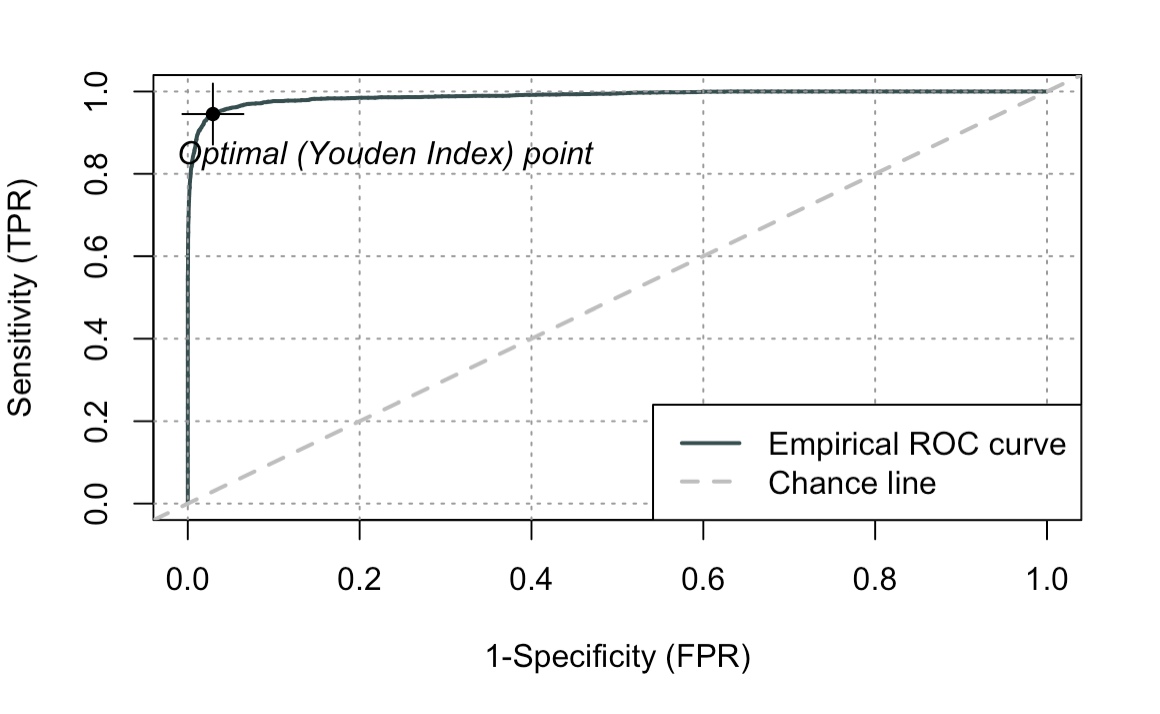
\includegraphics[width=0.45\textwidth]{log_1.jpeg}
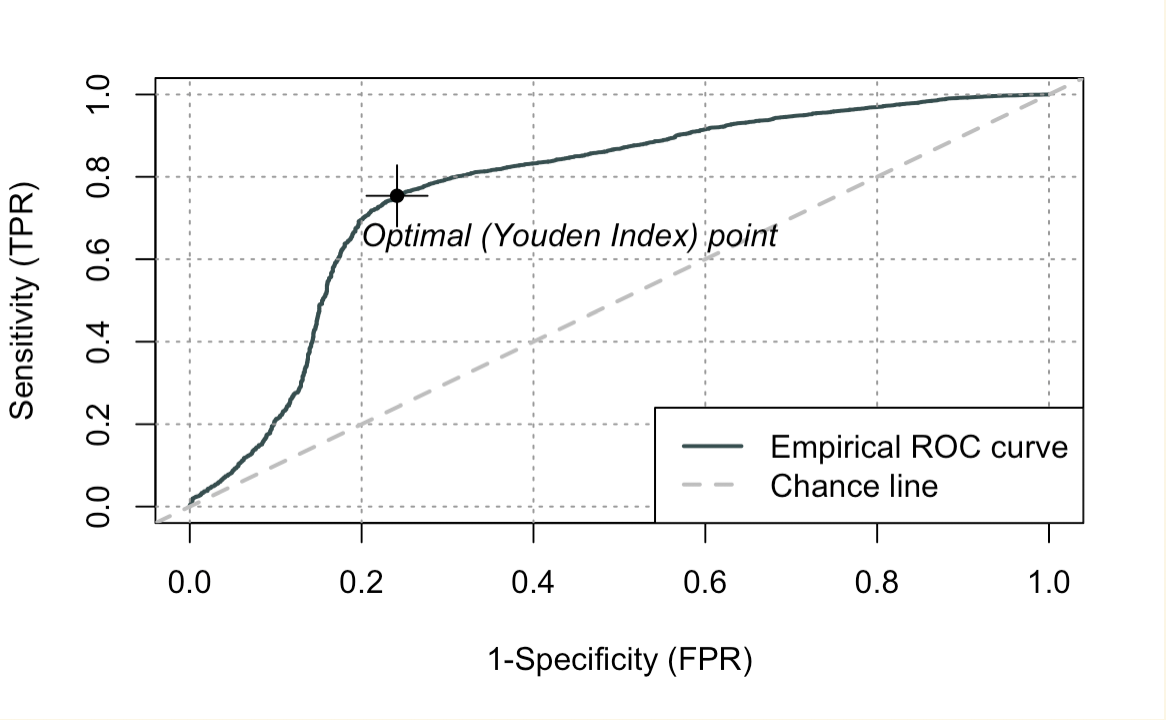
\includegraphics[width=0.45\textwidth]{log_2.jpeg}
\centering
\caption{ROC of Logistic Regression (Left: Method 1; Right: Method 2)}
\label{fig:3-1-2}
\centering
\end{figure}

We can see that the new cutoff provides a slightly better accuracy when the data is split by method 2, mainly because the shape of each ``slice'' in method 2 makes it hard for logistic regression to divide it with its normal cutoff, and a specialized cutoff will be helpful in this situation. 

Eventually, the test accuracy with method 1 is 0.6216 and 0.8702 for method 2.

\subsection{Support Vector Machine}

SVM works well with unstructured and semi-structured data like images. In this case, we find that SVM has similar performance with logistic regression. The CV accuracy of method 1 and method 2 with or without new cutoff are close to what of logistics classification. The optimal cutoff values method 1 and method 2 are 0.006530352 and 0.9856693 respectively, with test accuracy of 0.6837 and 0.8103.

\begin{figure}[h]
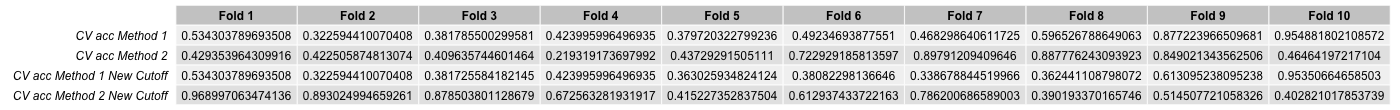
\includegraphics[width=\textwidth]{3-2-1.png}
\centering
\caption{Accuracy of SVM}
\label{fig:3-2-1}
\centering
\end{figure}

\begin{figure}[h]
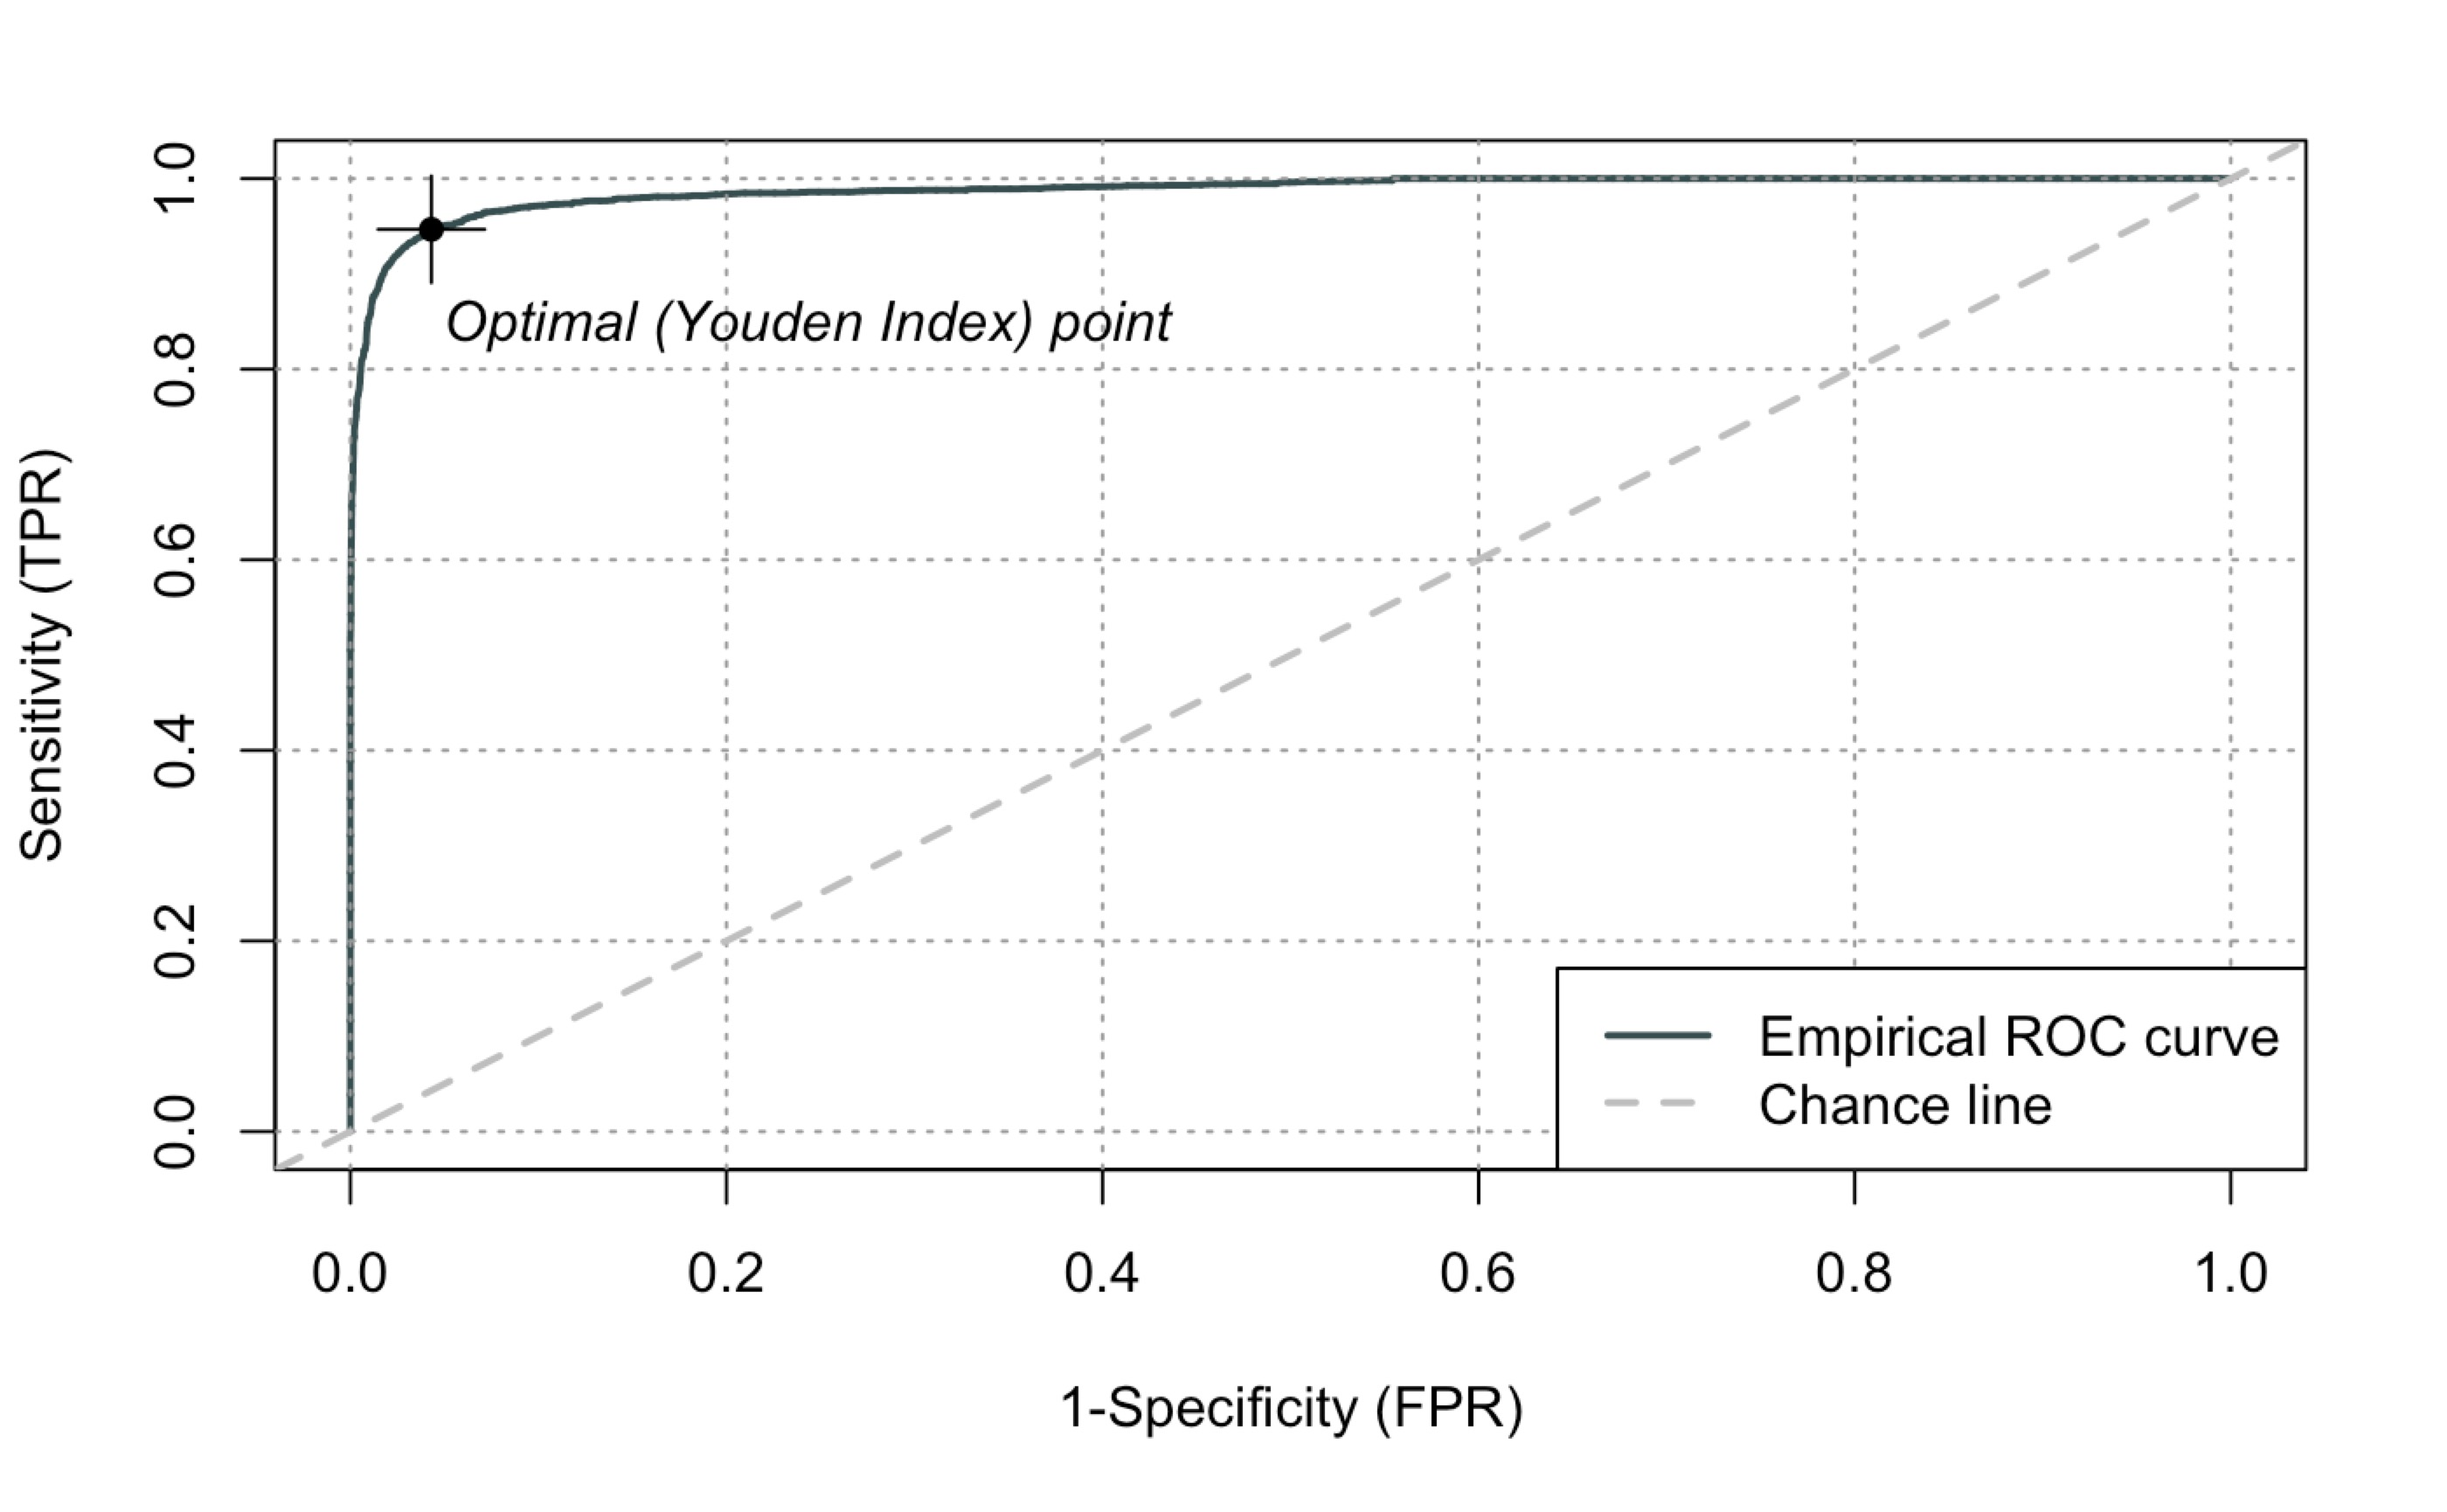
\includegraphics[width=0.45\textwidth]{svm_1.JPG}
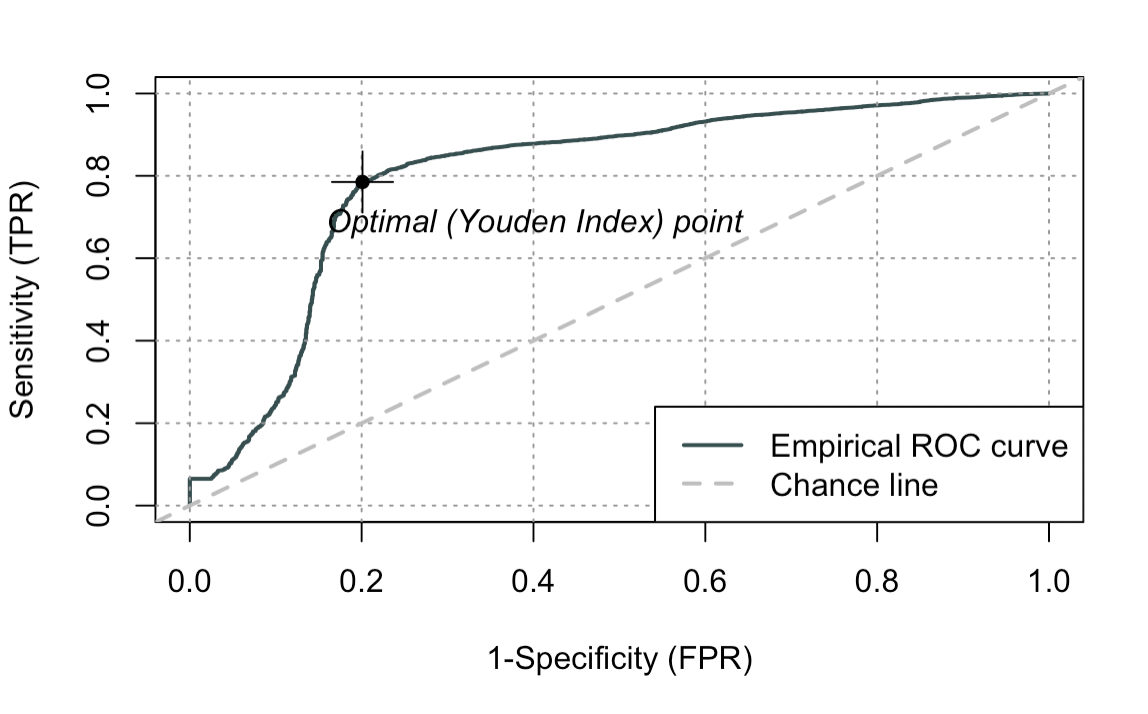
\includegraphics[width=0.45\textwidth]{svm_2.jpeg}
\caption{ROC of SVM (Left: Method 1; Right: Method 2)}
\label{fig:3-2-2}
\centering
\end{figure}



\subsection{Quadratic Discriminant Analysis}

From logistic regression, we know that a model might perform better if the lines that separate each cluster is non-linear. As a result, we ran a QDA model on the data. The cutoff values are also updated using a ROC curve shown in Figure \ref{fig:3-3-2}, which are 0.0139 and 0.9995 for method 1 and method 2 respectively. The resulting accuracy is shown in Figure \ref{fig:3-3-1}.

\begin{figure}[h]
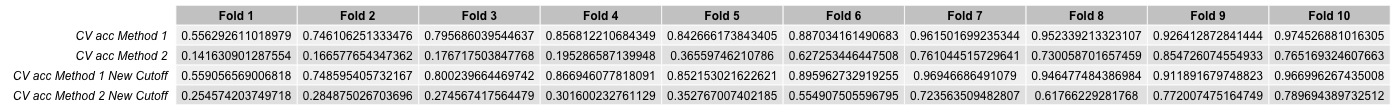
\includegraphics[width=\textwidth]{3-3-1.png}
\centering
\caption{Accuracy of QDA}
\label{fig:3-3-1}
\centering
\end{figure}

\begin{figure}[h]
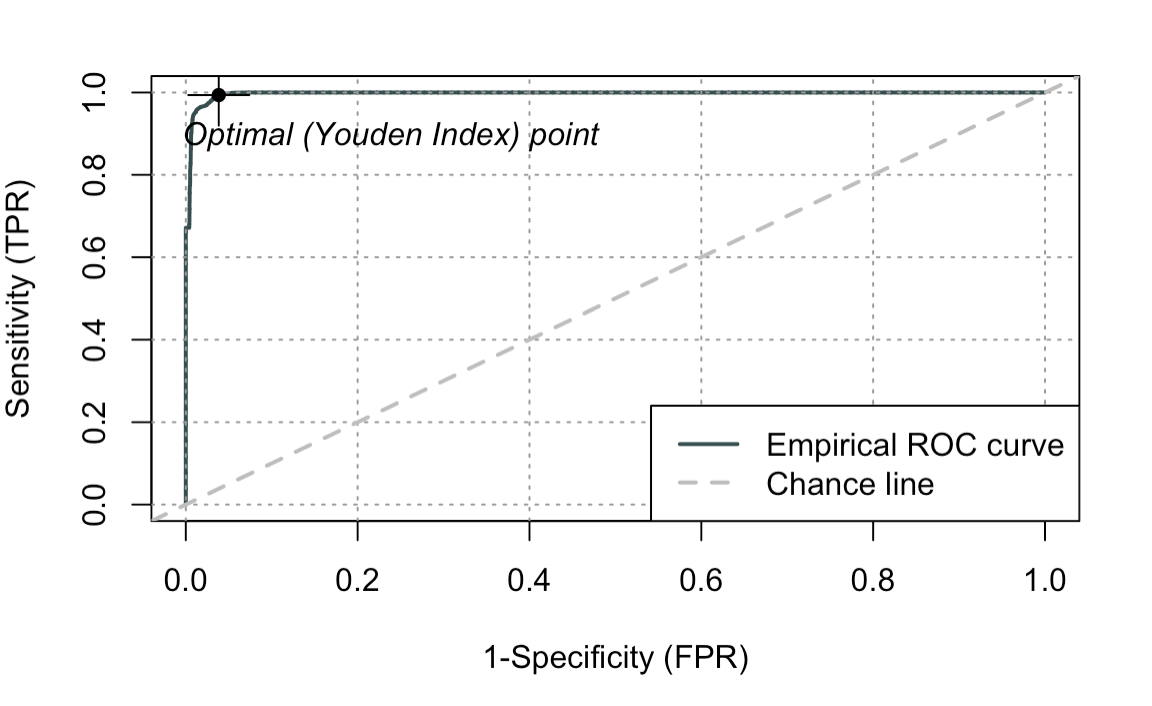
\includegraphics[width=0.45\textwidth]{qda_1.jpeg}
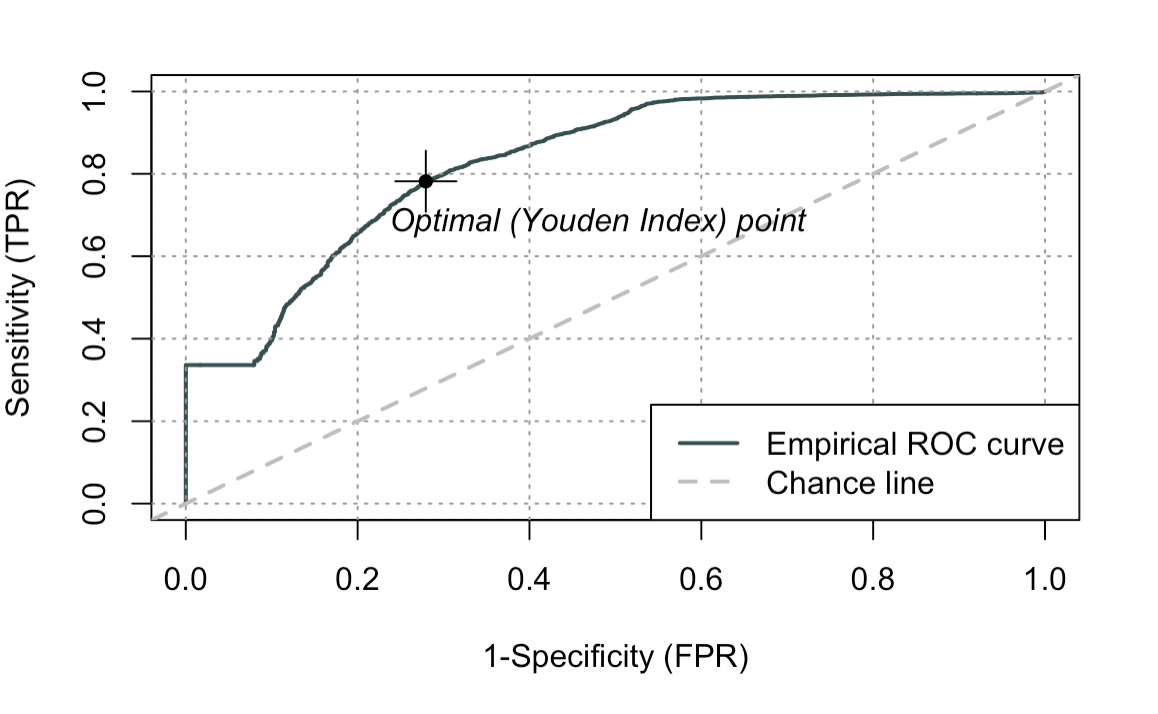
\includegraphics[width=0.45\textwidth]{qda_2.jpeg}
\centering
\caption{ROC of QDA (Left: Method 1; Right: Method 2)}
\label{fig:3-3-2}
\centering
\end{figure}

Similar to logistic regression, we can see that the new cutoff only improved accuracy for method 2, and method 1 generally has better CV accuracy. However, QDA did show a better result than logistic regression, which means that we are right about the dividing lines being non-linear. In the case of QDA, method 2 cutoff works better as it preserves the shape of the label chunks better.

The resulting test accuracy is 0.5045 and 0.903 for method 1 and 2 respectively. Surprisingly, QDA works better on method 2 with test data.


\subsection{Random Forest}

After all the parametric methods above, we have decided to run a method that introduces more variance for less bias, which is random forest, hoping that it can provide better accuracy and better results in method 2, as it doesn't divide data by lines. A ROC curve is also ran to choose for a better cutoff value as shown in Figure \ref{fig:3-4-2}, with accuracy shown in Figure \ref{fig:3-4-1}. The best cutoff value is 0.104 for method 1 and 0.85 for method 2.

\begin{figure}[h]
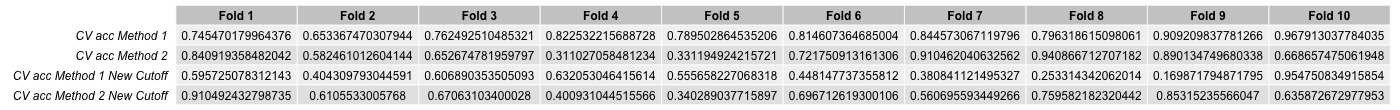
\includegraphics[width=\textwidth]{3-4-1.png}
\centering
\caption{Accuracy of Random Forest}
\label{fig:3-4-1}
\centering
\end{figure}

\begin{figure}[h]
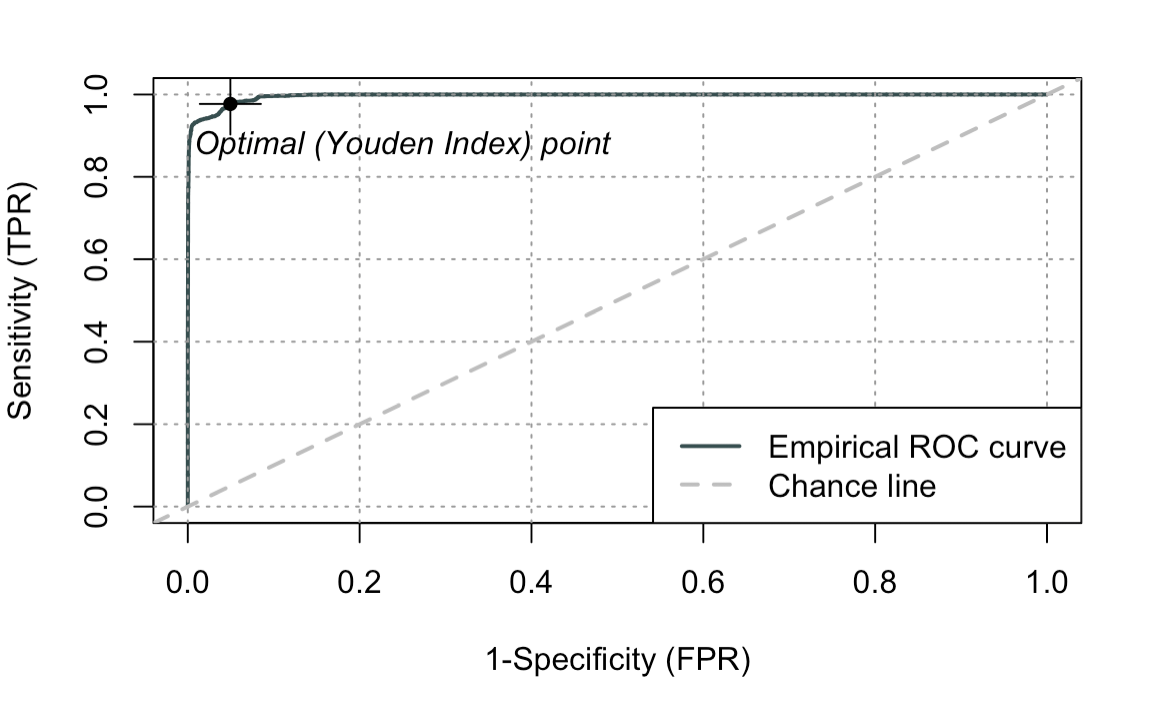
\includegraphics[width=0.45\textwidth]{rf_1.jpeg}
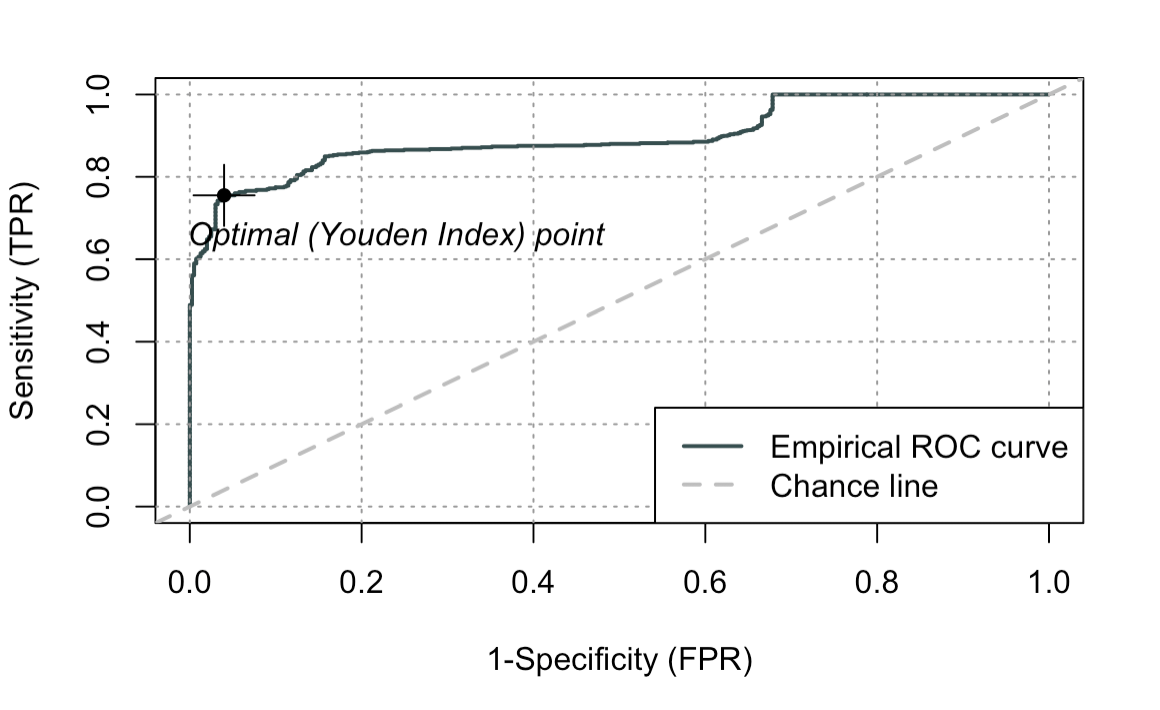
\includegraphics[width=0.45\textwidth]{rf_2.jpeg}
\centering
\caption{ROC of Random Forest (Left: Method 1; Right: Method 2)}
\label{fig:3-4-2}
\centering
\end{figure}

We can see the accuracy is generally better in random forest models compared to logistic, SVM and QDA. This could be due to the fact that random forest creates various decision trees to decrease bias. Similarly, the new cutoff value also helps with method 2's accuracy, mainly because of its unusual shape.

Random forest received a test accuracy of 0.6313 for method 1 and 0.9343 for method 2.


\subsection{ROC Comparison}

For each ROC plot, a cutoff value is chosen by Youden Index, or Youden's J Statistics. It has the following definition:

$
J = sensitivity + specificity - 1 = True Positive Rate - False Positive Rate 
$

From the plots for ROC shown previously, we can see that generally, method 1 has a nice ROC curve and AUC compared to method 2. This could be because the data is split in a ``weirder'' way in method 2. Within ROC plots for method 2, the ROC plot for random forest looks the best.

The cutoff point with maximum Youden Index is chosen as the new cutoff value for each model. With such new cutoff, we re-predict the labels of different models on validation set and training set. The results are shown in 3.1 - 3.4 section.

\subsection{Another Metric}


Figure \ref{fig:4-1-1} shows the accuracy in line plots. From the plot, we can see that the random forest model of the 8th fold using method 2 has the highest CV accuracy rate and test accuracy rate. Also, the plots show that the accuracy has a greater change after the cutoff value is updated on the models trained on data split by method 2 compared to method 1.

\begin{figure}[h]
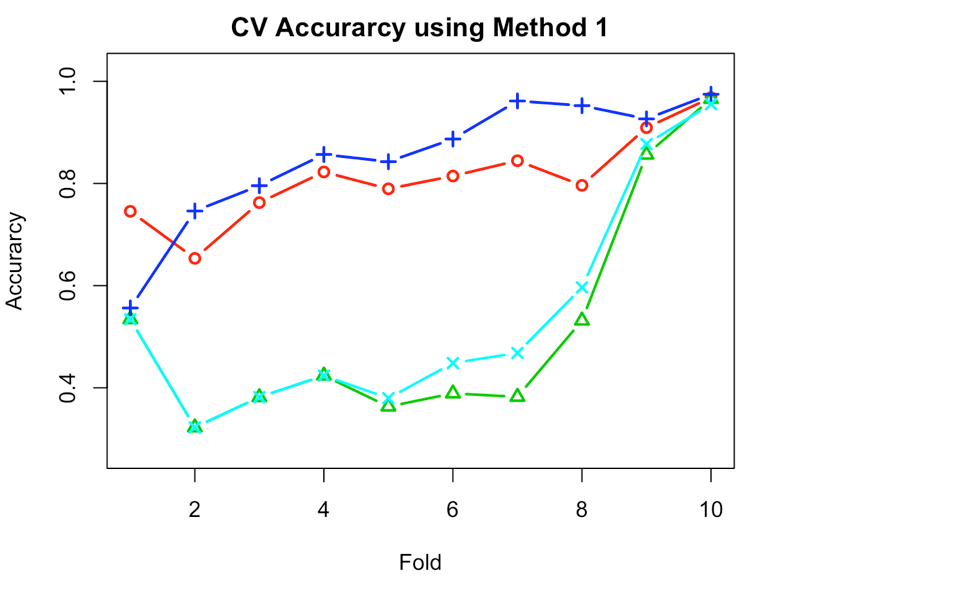
\includegraphics[width=0.22\textwidth]{raw_cv_1.png}
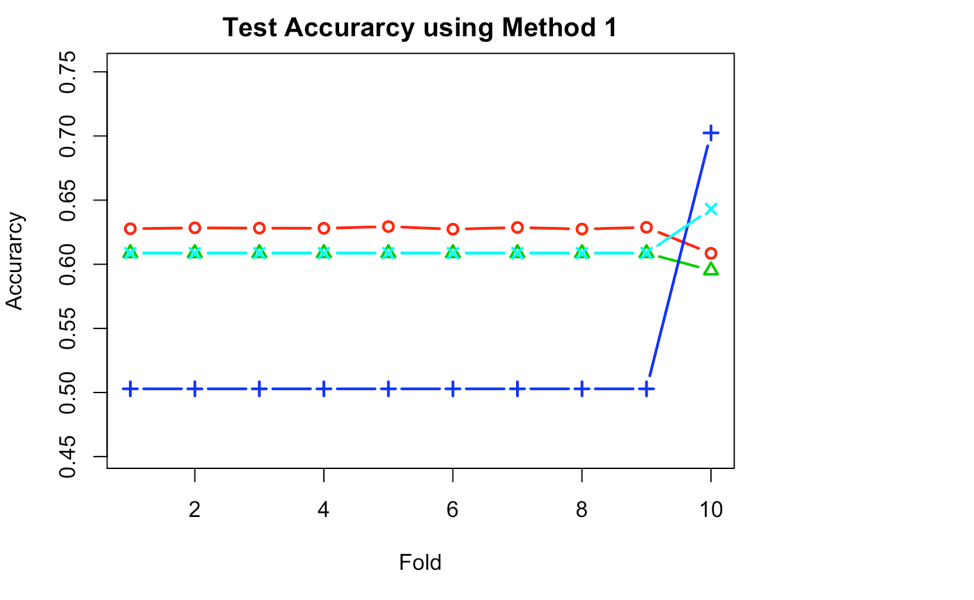
\includegraphics[width=0.22\textwidth]{raw_test_1.png}
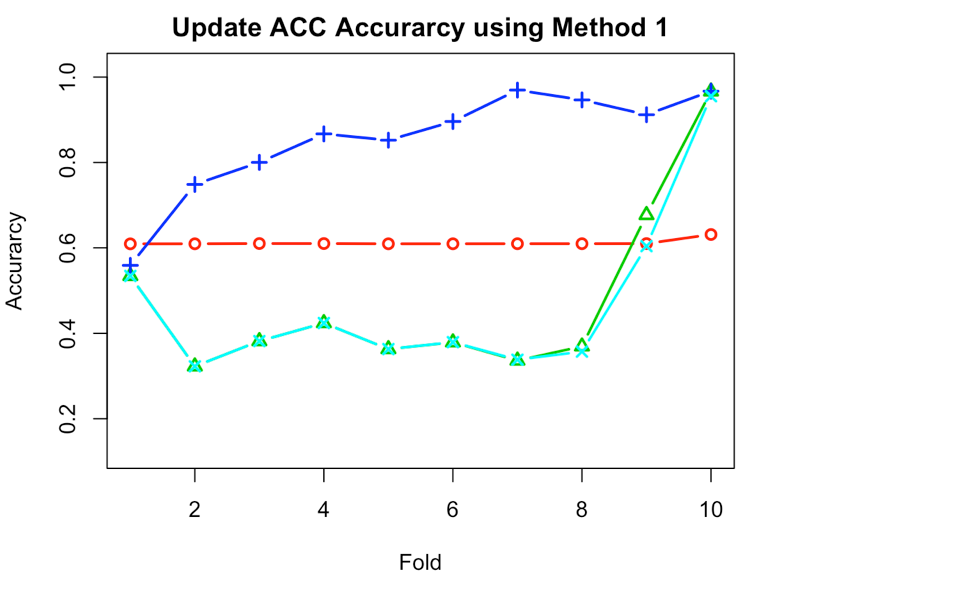
\includegraphics[width=0.22\textwidth]{update_cv_1.png}
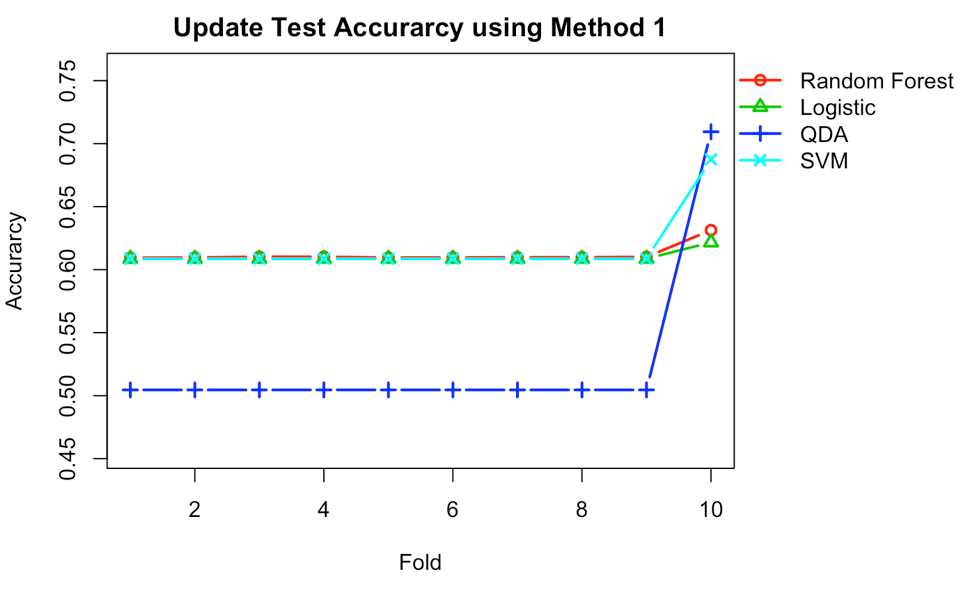
\includegraphics[width=0.22\textwidth]{update_test_1.png}
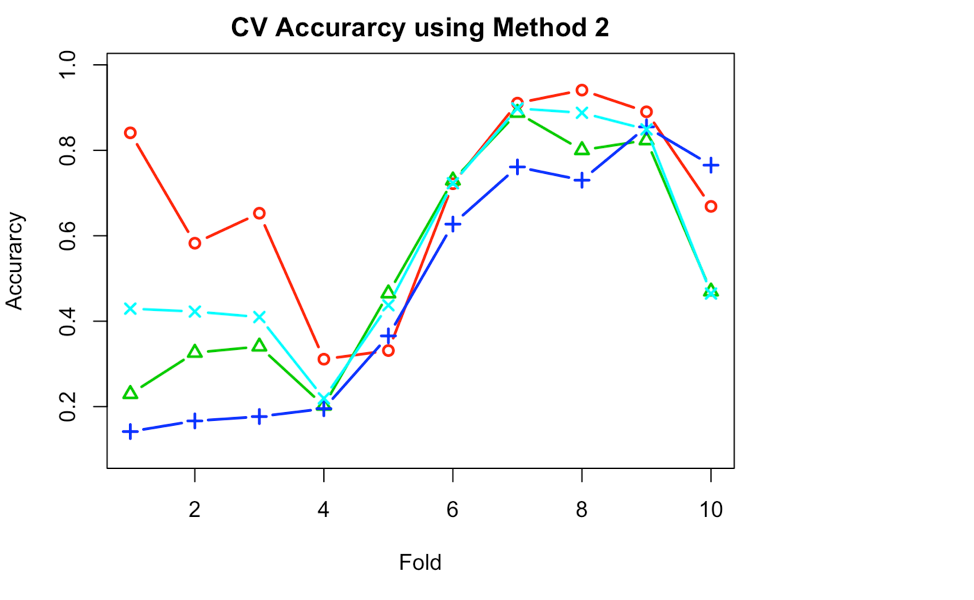
\includegraphics[width=0.22\textwidth]{raw_cv_2.png}
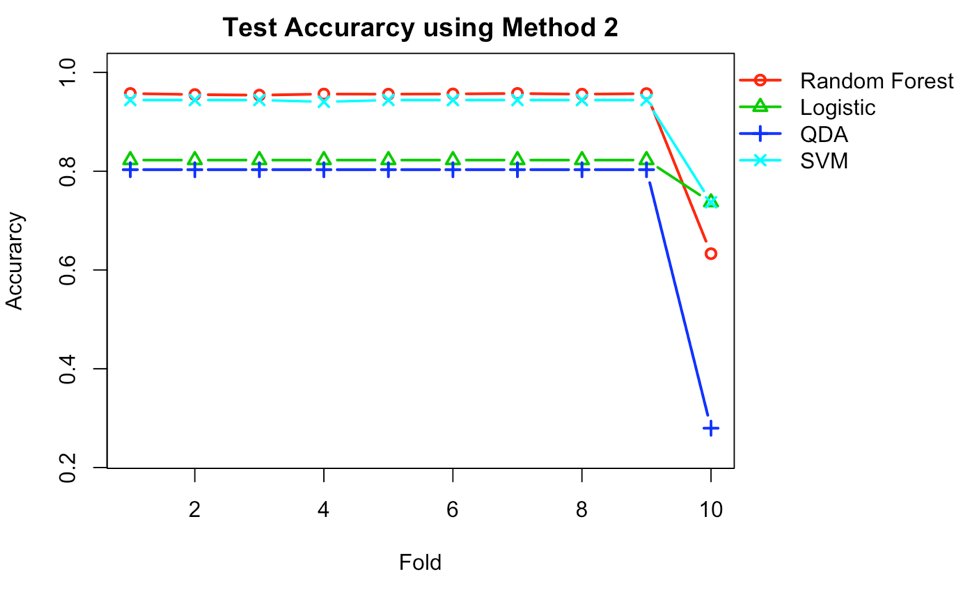
\includegraphics[width=0.22\textwidth]{raw_test_2.png}
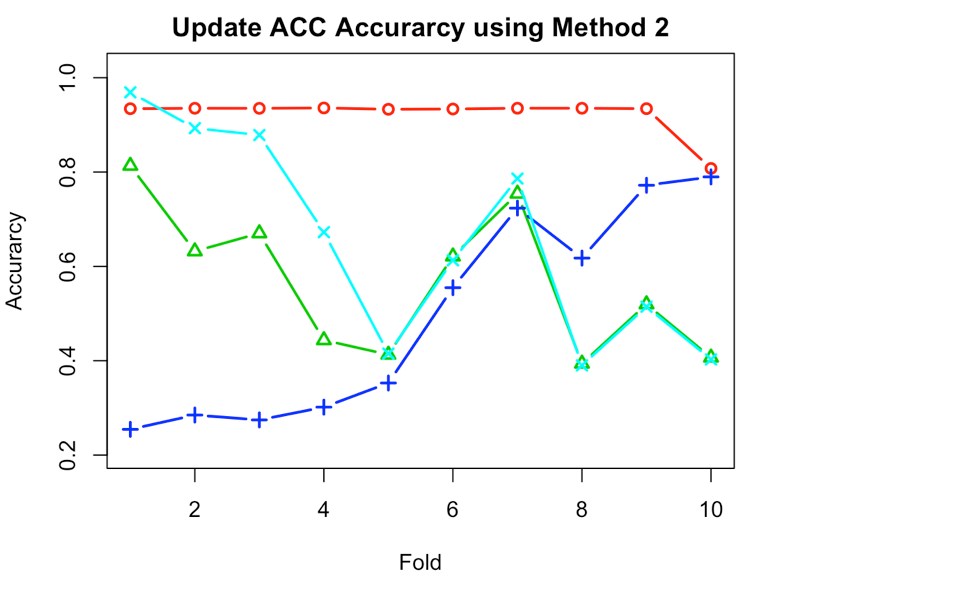
\includegraphics[width=0.22\textwidth]{update_cv_2.png}
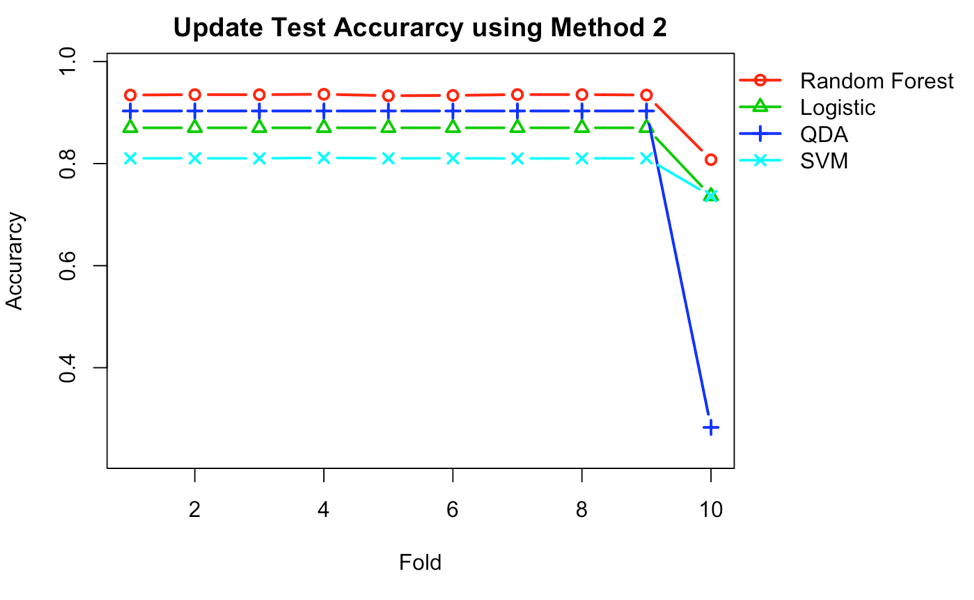
\includegraphics[width=0.22\textwidth]{update_test_2.png}
\centering
\caption{Comparison of Accuracy between Models}
\label{fig:4-1-1}
\centering
\end{figure}


\section{Diagnostics}

\subsection{Analysis on Random Forest}

Printing the model shows an OOB estimate of error rate 2.84\%. The training model fits the training data well. The class error of classify non-cloud is only 0.06. Compared to cloud, the model performs better on classifying non-clouds. The CV error and test error are 0.06 and 0.04 respectively. The variance importance plot indicates what variables had the greatest impact in the classification model. Three of ``best'' features are BF, NDAI, and DF, which are different from the conclusion we have from section 3.3. Since we do not have enough data on clouds (most of the data are labeled as non-cloud), the random forest model is unstable. Figure \ref{fig:4-1-2} also plots one of the trees using 5 variables in construction. It turned out to be 11 terminal nodes with misclassification error rate: 0.0493. 

\begin{figure}[h]
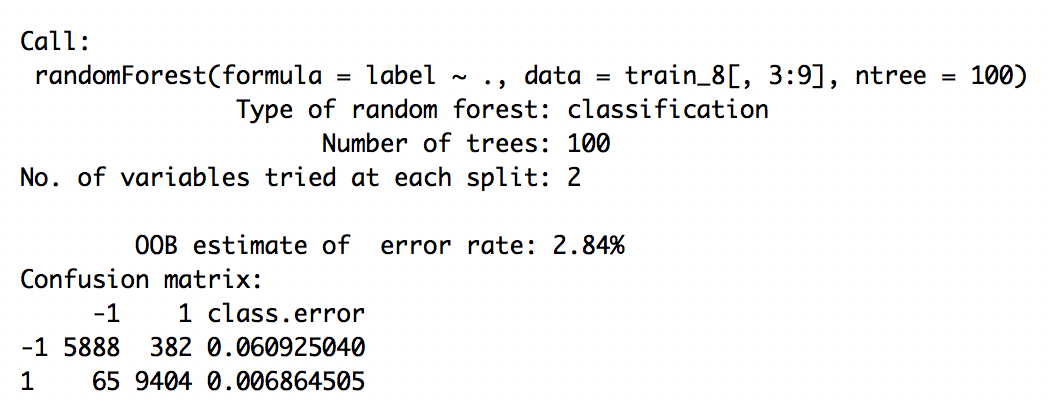
\includegraphics[width=0.59\textwidth]{4-1-1.png}
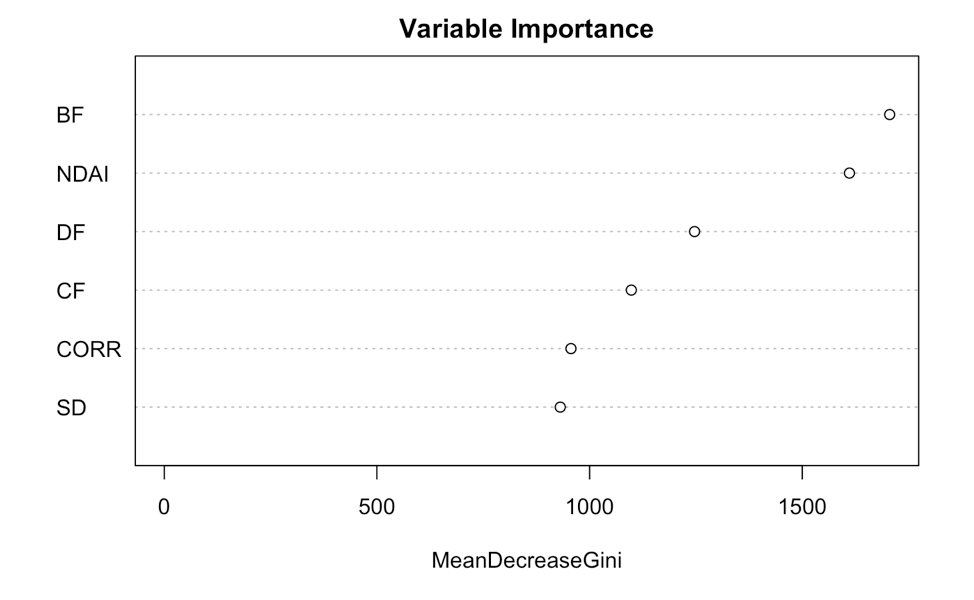
\includegraphics[width=0.4\textwidth]{4-1-2.png}
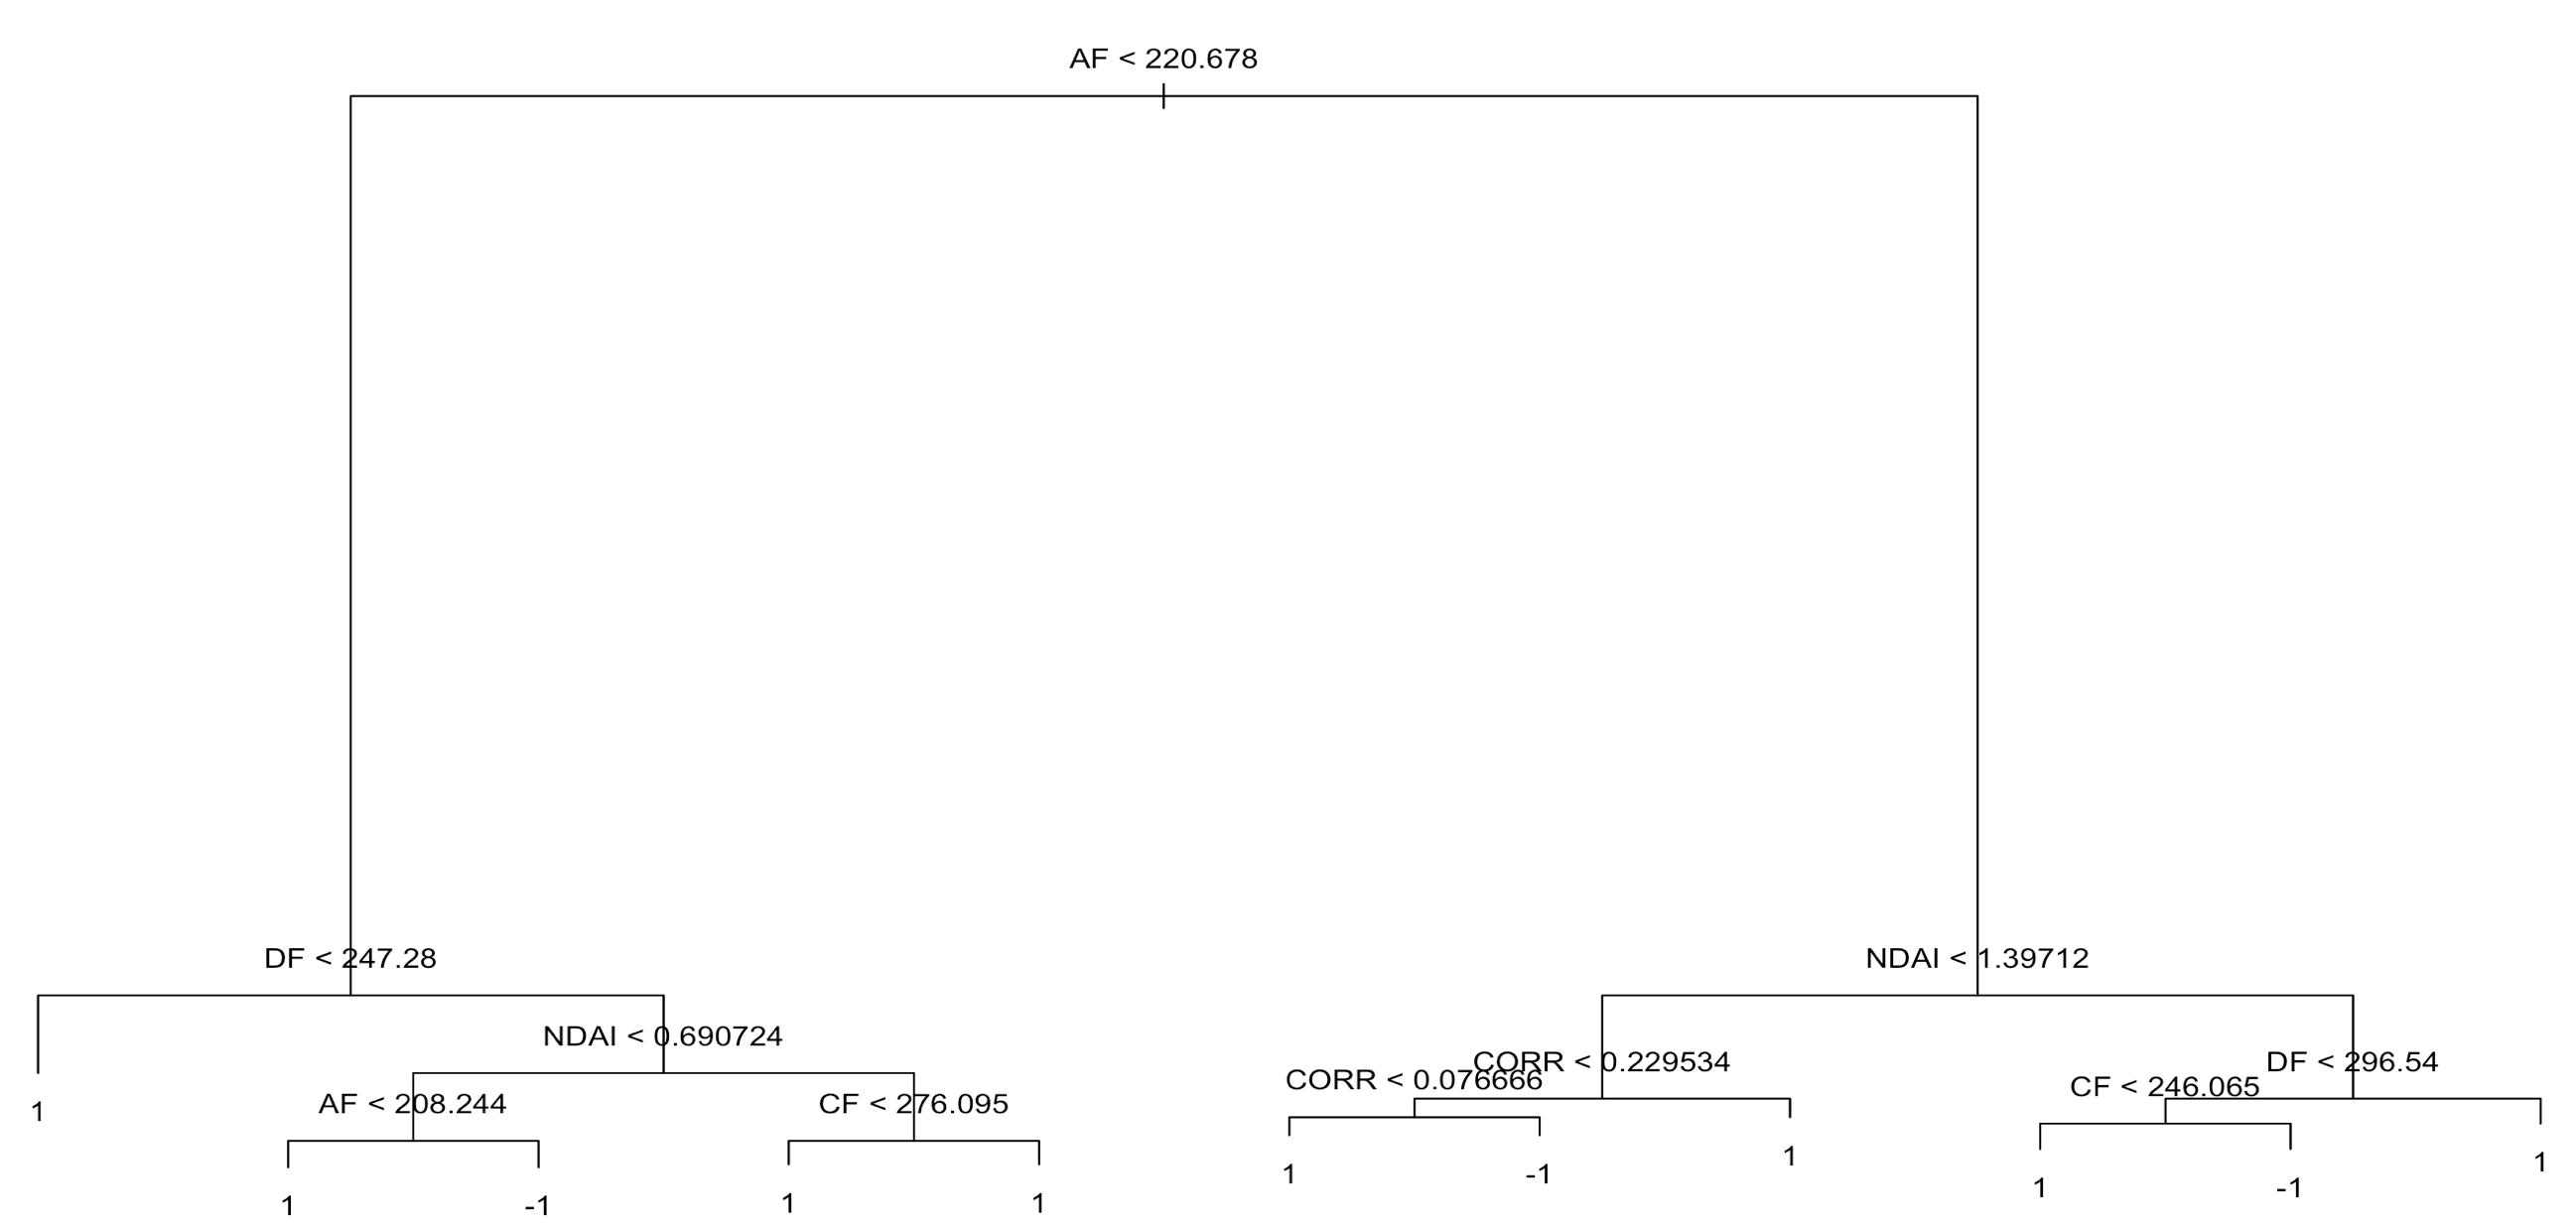
\includegraphics[width=0.6\textwidth]{4-1-3.png}
\centering
\caption{Random Forest of the 8th fold}
\label{fig:4-1-2}
\centering
\end{figure}

\subsection{Misclassification}

With the best classification model, we took its prediction result on test data, and computed a confusion matrix in Figure \ref{fig:4-2-1} left. From the confusion matrix, we can see that the model does a good job in predicting land, with most of its error in predicting clouds. In fact, its error in predicting clouds is almost 25\%!. This could be that unlike the similar, flat, icy land, clouds come in various shapes and forms, making it harder to predict.

\begin{figure}[h]
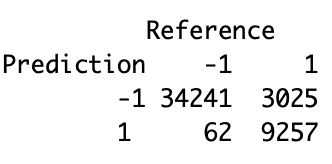
\includegraphics[width=0.2\textwidth]{4-2-1.jpeg}
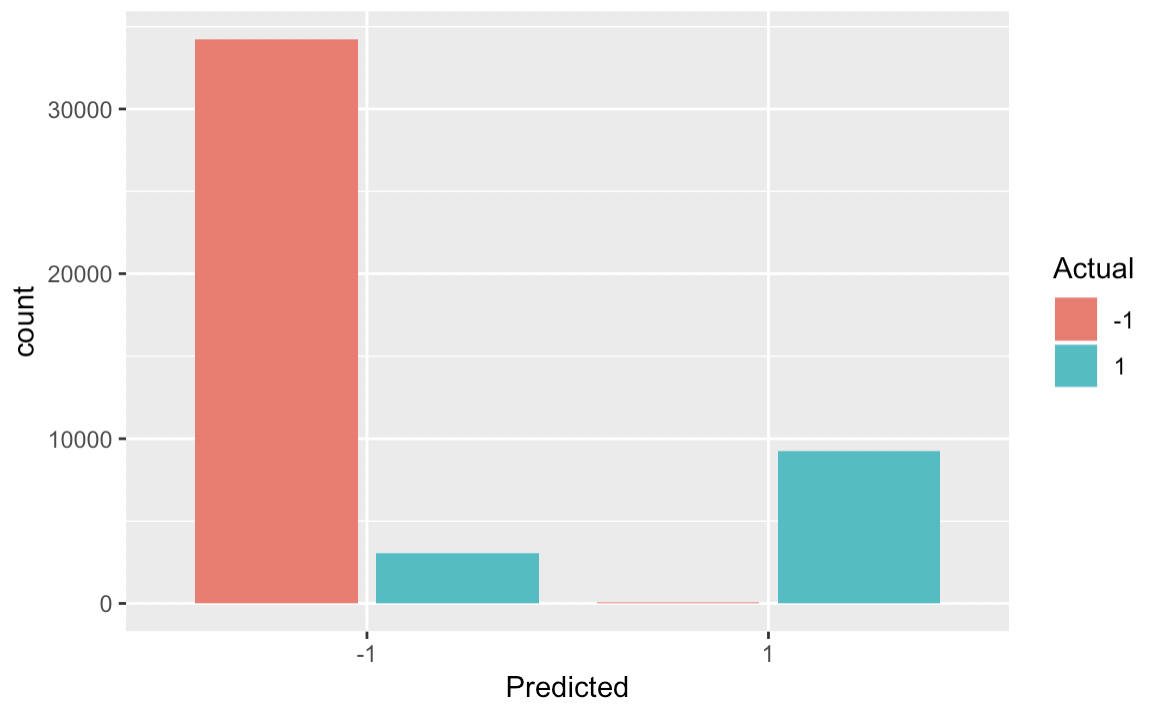
\includegraphics[width=0.4\textwidth]{4-2-2.jpeg}
\centering
\caption{Left: Confusion Matrix, Right: Histogram}
\label{fig:4-2-1}
\centering
\end{figure}

We further plotted out the location of classification error to see if it is easier to misclassify specific places compared to others. From the lower row of plots in Figure \ref{fig:4-2-2}, we can see that the misclassification errors mainly occur in the edge areas. This could be that at the edge of clouds, they become more transparent and harder to distinguish from land.

\begin{figure}[h]
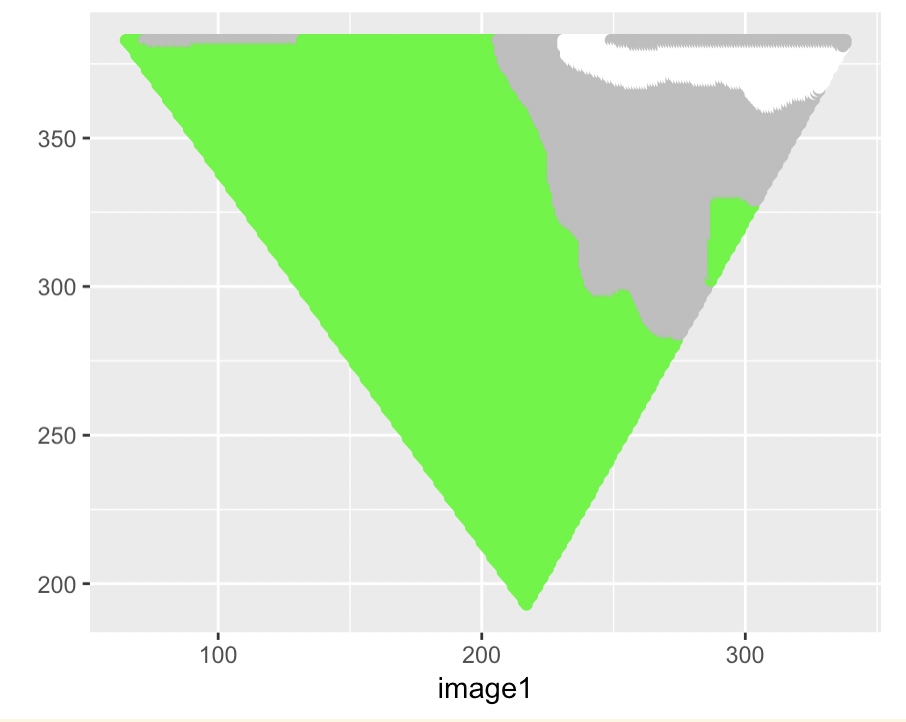
\includegraphics[width=0.28\textwidth]{4-2-3.jpeg}
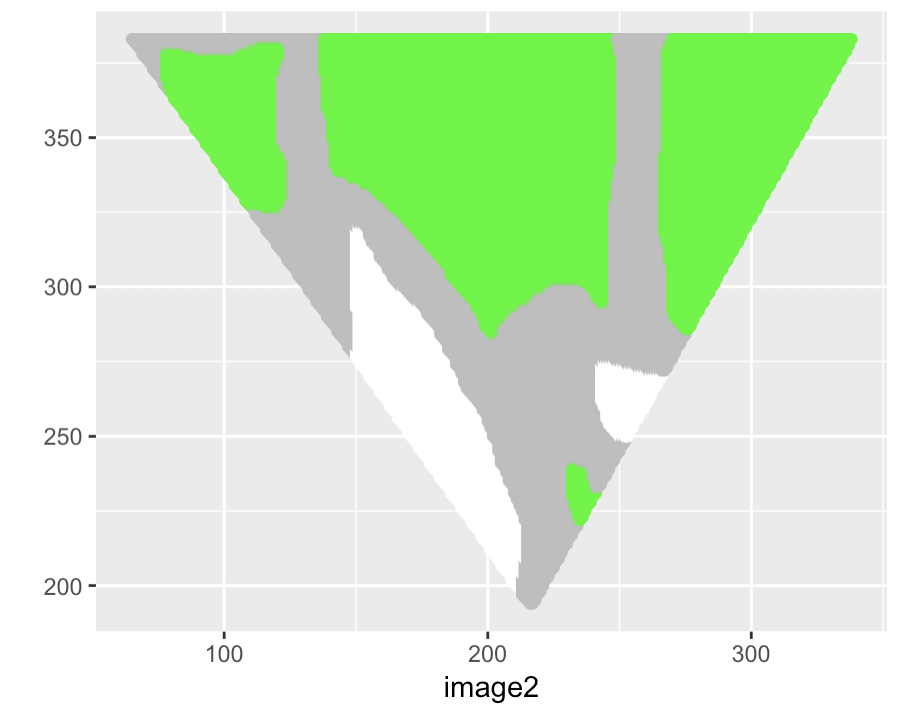
\includegraphics[width=0.28\textwidth]{4-2-4.jpeg}
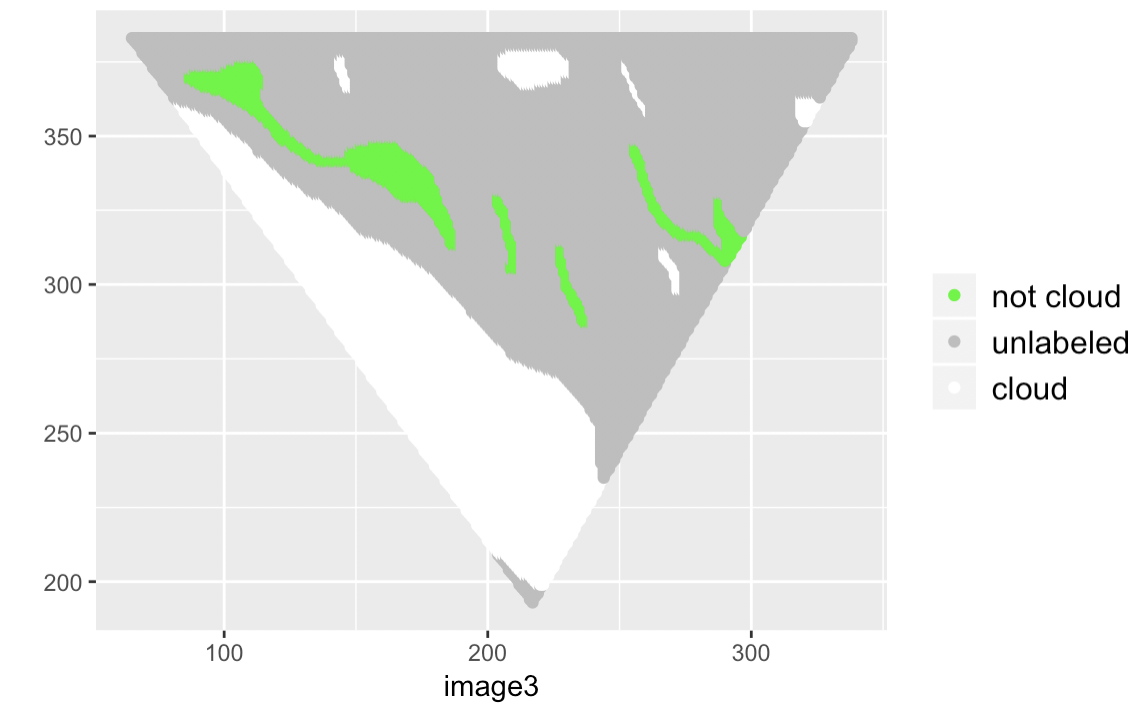
\includegraphics[width=0.35\textwidth]{4-2-5.jpeg}
\centering
\end{figure}

\begin{figure}[h]
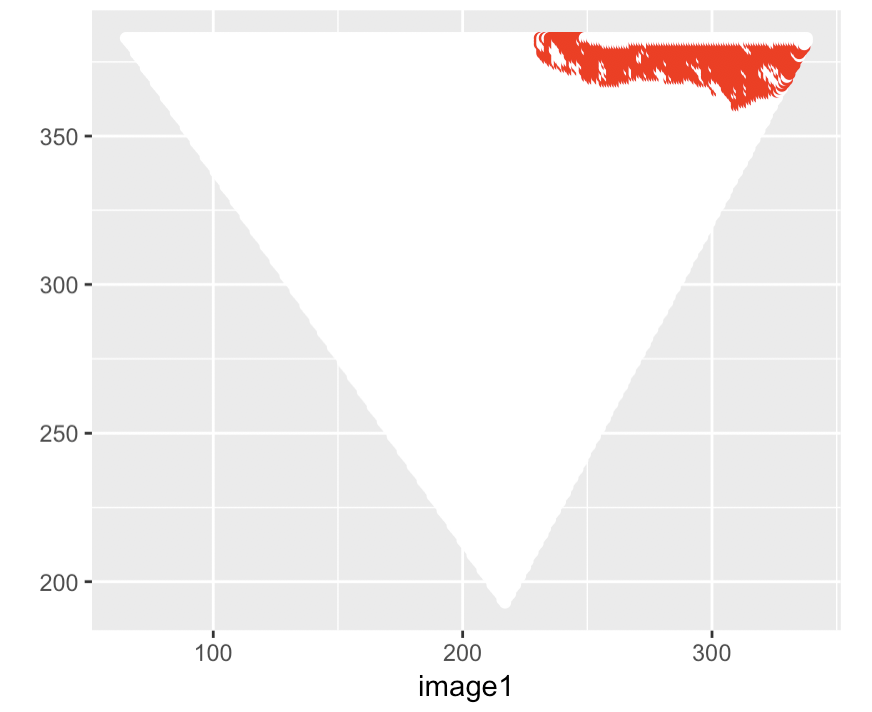
\includegraphics[width=0.28\textwidth]{4-2-6.jpeg}
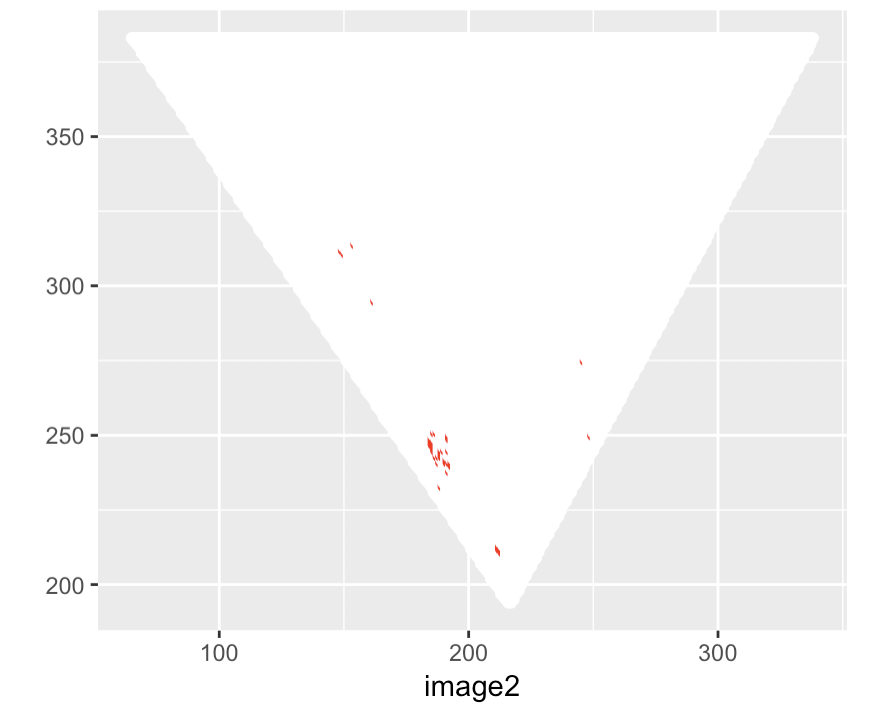
\includegraphics[width=0.28\textwidth]{4-2-7.jpeg}
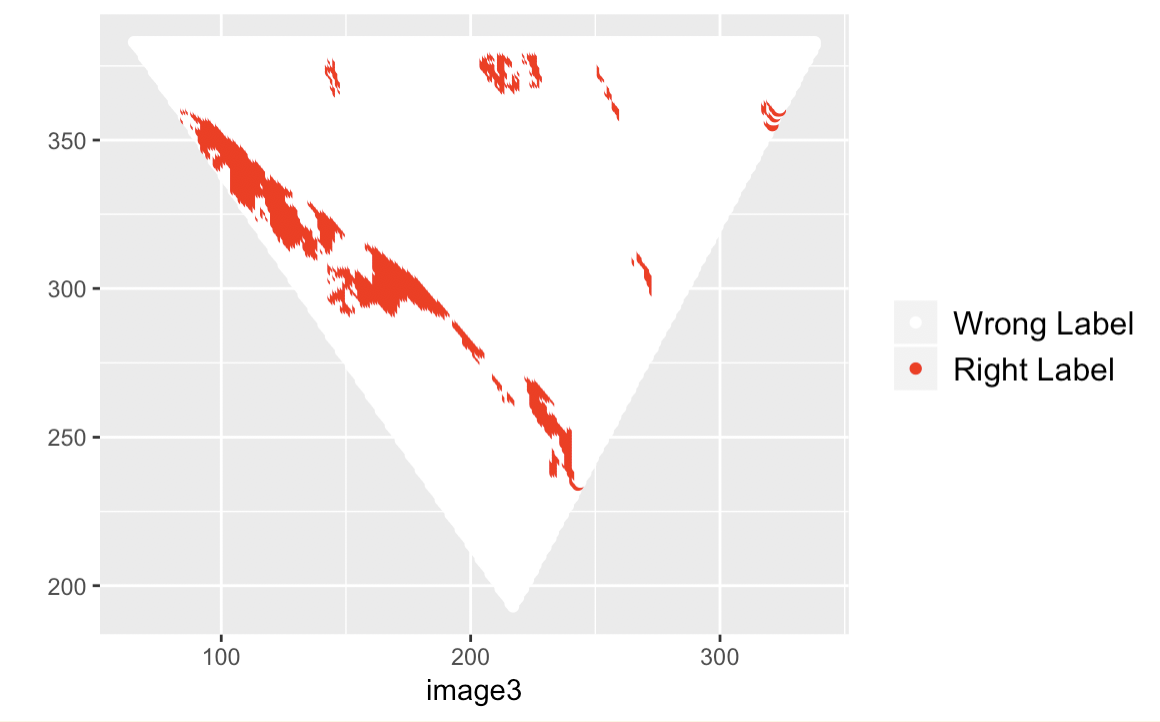
\includegraphics[width=0.36\textwidth]{4-2-8.jpeg}
\centering
\caption{Location of Misclassification}
\label{fig:4-2-2}
\centering
\end{figure}


\subsection{Better Classifier}

We find that non-parameter model, random forest, has better performance than parameter models, such as logistics, QDA, and SVM. K-nearest neighbors algorithm might be a better classifier because non-cloud and cloud appears in proximity with each other. We also need more data. We currently only have data from 3 images and the data is also unbalanced with high proportion of non-cloud pixels and low proportion of could pixels. Considering the classification performance mentioned in this paper, the new model might also suffer from the same problem: it can better classify the non-cloud labels than the cloud labels.


\subsection{Change in Data Splitting}

Figure \ref{fig:4-1-1} shows that using method 1 to split data gives lower CV and test accuracy. The reason might be that splitting data through method 2 ensures continuity in space. The long bars provided by method 1 splits data that have similar y coordinates but different x coordinates, while method 2 splits data that have both similar x and y coordinates together. Other methods that also has this property are to split into squares or rectangles. 

When inspecting the confusion matrix and the resulting histogram from using the same model on method 1 data (Figure \ref{fig:4-4-1}), we can see that this time, the model predicts most of the data to be clouds, which leads to a high accuracy in cloud prediction but low accuracy in land prediction. This is a further indicator that method 1 is not the optimal way for splitting the data.

\begin{figure}[h]
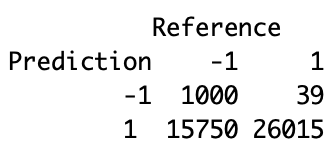
\includegraphics[width=0.2\textwidth]{4-4-1.jpeg}
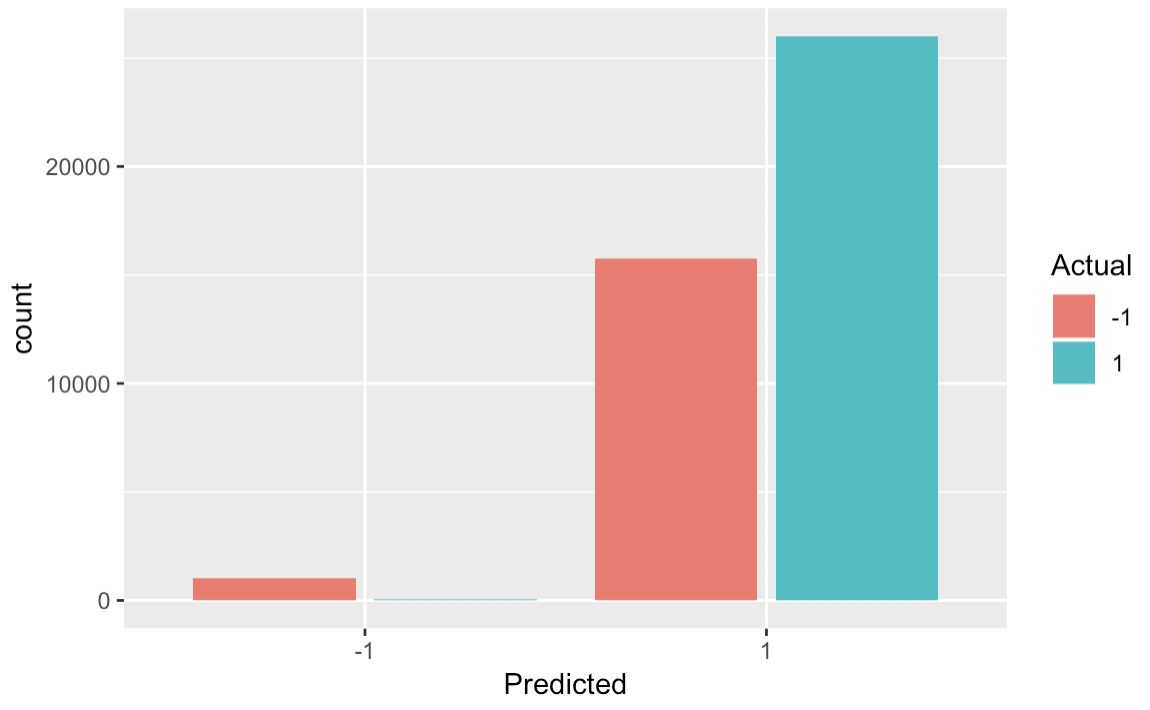
\includegraphics[width=0.4\textwidth]{4-4-2.jpeg}
\centering
\caption{Left: Confusion Matrix, Right: Histogram}
\label{fig:4-4-1}
\centering
\end{figure}


\subsection{Conclusion}

The four classification methods perform well in classifying the non-cloud labels compared to cloud labels. Among the four models, random forest provides the best result, but still suffer from the same problem. Having more unskewed data to train random forest or switch to KNN might provide better results. In terms of misclassification error, it usually occurs on the edge of cloud area.  


\section{Reproducibility}

The full code (including R code and latex code) can be seen in this github repository:

https://github.com/estherwu211/stat154\_project2

The README.md file provides details on how to run the code with new image data.


\section{Acknowledgment}
Work is divided equally among authors, and both authors participated in each step of the analysis.


\end{document}